% ******************************* PhD Thesis Template **************************
% Please have a look at the README.md file for info on how to use the template

\documentclass[a4paper,11pt,times,print,oneside,authoryear,custommargin]{Classes/PhDThesisPSnPDF}

% ******************************************************************************
% ******************************* Class Options ********************************
% *********************** See README for more details **************************
% ******************************************************************************

% `a4paper'(The University of Cambridge PhD thesis guidelines recommends a page
% size a4 - default option) or `a5paper': A5 Paper size is also allowed as per
% the Cambridge University Engineering Deparment guidelines for PhD thesis
%
% `11pt' or `12pt'(default): Font Size 10pt is NOT recommended by the University
% guidelines
%
% `oneside' or `twoside'(default): Printing double side (twoside) or single
% side.
%
% `print': Use `print' for print version with appropriate margins and page
% layout. Leaving the options field blank will activate Online version.
%
% `index': For index at the end of the thesis
%
% `draftclassic': For draft mode without loading any images (same as draft in book)
%
% `draft': Special draft mode with line numbers, images, and water mark with
% timestamp and custom text. Position of the text can also be modified.
%
% `abstract': To generate only the title page and abstract page with
% dissertation title and name, to submit to the Student Registry
%
% `chapter`: This option enables only the specified chapter and it's references
%  Useful for review and corrections.
%
% ************************* Custom Page Margins ********************************
%
% `custommargin`: Use `custommargin' in options to activate custom page margins,
% which can be defined in the preamble.tex. Custom margin will override
% print/online margin setup.
%
% *********************** Choosing the Fonts in Class Options ******************
%
% `times' : Times font with math support. (The Cambridge University guidelines
% recommend using times)
%
% `fourier': Utopia Font with Fourier Math font (Font has to be installed)
%            It's a free font.
%
% `customfont': Use `customfont' option in the document class and load the
% package in the preamble.tex
%
% default or leave empty: `Latin Modern' font will be loaded.
%
% ********************** Choosing the Bibliography style ***********************
%
% `authoryear': For author-year citation eg., Krishna (2013)
%
% `numbered': (Default Option) For numbered and sorted citation e.g., [1,5,2]
%
% `custombib': Define your own bibliography style in the `preamble.tex' file.
% \RequirePackage[square, sort, numbers, authoryear]{natbib}
%              This can be also used to load biblatex instead of natbib
%              (See Preamble)
%
% **************************** Choosing the Page Style *************************
%
% `default (leave empty)': For Page Numbers in Header (Left Even, Right Odd) and
% Chapter Name in Header (Right Even) and Section Name (Left Odd). Blank Footer.
%
% `PageStyleI': Chapter Name next & Page Number on Even Side (Left Even).
% Section Name & Page Number in Header on Odd Side (Right Odd). Footer is empty.
%
% `PageStyleII': Chapter Name on Even Side (Left Even) in Header. Section Number
% and Section Name in Header on Odd Side (Right Odd). Page numbering in footer

% Uncomment to change page style
%\pagestyle{PageStyleII}

% ********************************** Preamble **********************************
% Preamble: Contains packages and user-defined commands and settings
% ******************************************************************************
% ****************************** Custom Margin *********************************

% Add `custommargin' in the document class options to use this section
% Set {innerside margin / outerside margin / topmargin / bottom margin}  and
% other page dimensions
\ifsetCustomMargin
  \RequirePackage[left=37mm,right=30mm,top=35mm,bottom=30mm]{geometry}
  \setFancyHdr % To apply fancy header after geometry package is loaded
\fi

% Add spaces between paragraphs
%\setlength{\parskip}{0.5em}
% Ragged bottom avoids extra whitespaces between paragraphs
\raggedbottom
% To remove the excess top spacing for enumeration, list and description
%\usepackage{enumitem}
%\setlist[enumerate,itemize,description]{topsep=0em}

% *****************************************************************************
% ******************* Fonts (like different typewriter fonts etc.)*************

% Add `customfont' in the document class option to use this section

\ifsetCustomFont
  % Set your custom font here and use `customfont' in options. Leave empty to
  % load computer modern font (default LaTeX font).
  %\RequirePackage{helvet}

  % For use with XeLaTeX
  %  \setmainfont[
  %    Path              = ./libertine/opentype/,
  %    Extension         = .otf,
  %    UprightFont = LinLibertine_R,
  %    BoldFont = LinLibertine_RZ, % Linux Libertine O Regular Semibold
  %    ItalicFont = LinLibertine_RI,
  %    BoldItalicFont = LinLibertine_RZI, % Linux Libertine O Regular Semibold Italic
  %  ]
  %  {libertine}
  %  % load font from system font
  %  \newfontfamily\libertinesystemfont{Linux Libertine O}
\fi

% *****************************************************************************
% **************************** Custom Packages ********************************

% ************************* Algorithms and Pseudocode **************************

%\usepackage{algpseudocode}


% ********************Captions and Hyperreferencing / URL **********************

% Captions: This makes captions of figures use a boldfaced small font.
%\RequirePackage[small,bf]{caption}

\RequirePackage[labelsep=space,tableposition=top]{caption}
\renewcommand{\figurename}{Fig.} %to support older versions of captions.sty


% *************************** Graphics and figures *****************************

%\usepackage{rotating}
%\usepackage{wrapfig}

% Uncomment the following two lines to force Latex to place the figure.
% Use [H] when including graphics. Note 'H' instead of 'h'
%\usepackage{float}
%\restylefloat{figure}

% Subcaption package is also available in the sty folder you can use that by
% uncommenting the following line
% This is for people stuck with older versions of texlive
%\usepackage{sty/caption/subcaption}
\usepackage{subcaption}

% ********************************** Tables ************************************
\usepackage{booktabs} % For professional looking tables
\usepackage{multirow}

%\usepackage{multicol}
%\usepackage{longtable}
%\usepackage{tabularx}


% *********************************** SI Units *********************************
\usepackage{siunitx} % use this package module for SI units


% ******************************* Line Spacing *********************************

% Choose linespacing as appropriate. Default is one-half line spacing as per the
% University guidelines

% \doublespacing
% \onehalfspacing
% \singlespacing


% ************************ Formatting / Footnote *******************************

% Don't break enumeration (etc.) across pages in an ugly manner (default 10000)
%\clubpenalty=500
%\widowpenalty=500

%\usepackage[perpage]{footmisc} %Range of footnote options


% *****************************************************************************
% *************************** Bibliography  and References ********************

%\usepackage{cleveref} %Referencing without need to explicitly state fig /table

% Add `custombib' in the document class option to use this section
\ifuseCustomBib
   \RequirePackage[square, sort, numbers, authoryear]{natbib} % CustomBib

% If you would like to use biblatex for your reference management, as opposed to the default `natbibpackage` pass the option `custombib` in the document class. Comment out the previous line to make sure you don't load the natbib package. Uncomment the following lines and specify the location of references.bib file

%\RequirePackage[backend=biber, style=numeric-comp, citestyle=numeric, sorting=nty, natbib=true]{biblatex}
%\bibliography{References/references} %Location of references.bib only for biblatex

\fi

% changes the default name `Bibliography` -> `References'
\renewcommand{\bibname}{References}


% ******************************************************************************
% ************************* User Defined Commands ******************************
% ******************************************************************************

% *********** To change the name of Table of Contents / LOF and LOT ************

%\renewcommand{\contentsname}{My Table of Contents}
%\renewcommand{\listfigurename}{My List of Figures}
%\renewcommand{\listtablename}{My List of Tables}


% ********************** TOC depth and numbering depth *************************

\setcounter{secnumdepth}{2}
\setcounter{tocdepth}{2}


% ******************************* Nomenclature *********************************

% To change the name of the Nomenclature section, uncomment the following line

%\renewcommand{\nomname}{Symbols}


% ********************************* Appendix ***********************************

% The default value of both \appendixtocname and \appendixpagename is `Appendices'. These names can all be changed via:

%\renewcommand{\appendixtocname}{List of appendices}
%\renewcommand{\appendixname}{Appndx}

% *********************** Configure Draft Mode **********************************

% Uncomment to disable figures in `draft'
%\setkeys{Gin}{draft=true}  % set draft to false to enable figures in `draft'

% These options are active only during the draft mode
% Default text is "Draft"
%\SetDraftText{DRAFT}

% Default Watermark location is top. Location (top/bottom)
%\SetDraftWMPosition{bottom}

% Draft Version - default is v1.0
%\SetDraftVersion{v1.1}

% Draft Text grayscale value (should be between 0-black and 1-white)
% Default value is 0.75
%\SetDraftGrayScale{0.8}


% ******************************** Todo Notes **********************************
%% Uncomment the following lines to have todonotes.

%\ifsetDraft
%	\usepackage[colorinlistoftodos]{todonotes}
%	\newcommand{\mynote}[1]{\todo[author=kks32,size=\small,inline,color=green!40]{#1}}
%\else
%	\newcommand{\mynote}[1]{}
%	\newcommand{\listoftodos}{}
%\fi

% Example todo: \mynote{Hey! I have a note}

% *****************************************************************************
% ******************* Better enumeration my MB*************
\usepackage{enumitem}


% ************************ Thesis Information & Meta-data **********************
% Thesis title and author information, refernce file for biblatex
% ************************ Thesis Information & Meta-data **********************
%% The title of the thesis
\title{Smart Contracts for e-Learning}
%\texorpdfstring is used for PDF metadata. Usage:
%\texorpdfstring{LaTeX_Version}{PDF Version (non-latex)} eg.,
%\texorpdfstring{$sigma$}{sigma}

%% Subtitle (Optional)
% \subtitle{Using the CUED template}

%% The full name of the author
\author{Tsz Yiu Lam}

%% Department (eg. Department of Engineering, Maths, Physics)
\dept{Department of Computer Science}

%% University and Crest
\university{Brunel University London}
% Crest minimum should be 30mm.
\crest{
\includegraphics[width=0.5\textwidth]{BUL_LOGO_POS_RGB}}


%% Supervisor (optional)
%% for multiple supervisors, append each supervisor with the \newline command
\supervisor{Dr. Brijesh Dongol} %\newline
%Prof. C.D. Supervisor}

%% Supervisor Role (optional) - Supervisor (default) or advisor
\supervisorrole{\textbf{Supervisor: }}
%% if no title is desired:
% \supervisorrole{}

%% Supervisor line width: required to align supervisors
\supervisorlinewidth{0.35\textwidth}

%% Advisor (optional)
%% for multiple advisors, append each advisor with the \newline command
%\advisor{Dr. A. Advisor\newline
%Dr. B. Advisor}
     
%% Advisor Role (optional) - Advisor (default) or leave empty
% \advisorrole{Advisors: }
%% if no title is required
% \advisorrole{}

%% Advisor line width: required to align supervisors
%\advisorlinewidth{0.25\textwidth}


%% You can redefine the submission text:
% Default as per the University guidelines:
% ``This dissertation is submitted for the degree of''
%\renewcommand{\submissiontext}{change the default text here if needed}

%% Full title of the Degree
\degreetitle{Bachelor of Science in Business Computing}

%% College affiliation (optional)
%\college{College of Engineering, Design and Physical Sciences}

%% Submission date
% Default is set as {\monthname[\the\month]\space\the\year}
\degreedate{March 2018} 

%% Meta information
\subject{LaTeX} \keywords{{LaTeX} {Undergraduate Project} {CEDPS} {Brunel University London}}


% ***************************** Abstract Separate ******************************
% To printout only the titlepage and the abstract with the PhD title and the
% author name for submission to the Student Registry, use the `abstract' option in
% the document class.

\ifdefineAbstract
 \pagestyle{empty}
 \includeonly{Declaration/declaration, Abstract/abstract}
\fi

% ***************************** Chapter Mode ***********************************
% The chapter mode allows user to only print particular chapters with references
% Title, Contents, Frontmatter are disabled by default
% Useful option to review a particular chapter or to send it to supervisior.
% To use choose `chapter' option in the document class

\ifdefineChapter
 \includeonly{Chapter5/chapter5}
\fi

% ******************************** Front Matter ********************************
\begin{document}

\frontmatter

\maketitle

\begin{spacing}{1.5}
% ******************************* Thesis Dedidcation ********************************

\begin{dedication} 

I would like to dedicate this thesis to my loving parents \dots

\end{dedication}


% ************************** Thesis Abstract *****************************
% Use `abstract' as an option in the document class to print only the titlepage and the abstract.
\begin{abstract}
This is where you write your abstract ...
\end{abstract}

% ************************** Thesis Acknowledgements **************************

\begin{acknowledgements}      

\begin{center}
I would like to dedicate this paper to Mum, Dad, Vivien, Viviana, and Jorden.\\
\end{center}

The formatting of this report is done with Krishna Kumar's Cambridge University Engineering Department PhD thesis 
LaTeX template, and with reference to a Microsoft Word template provided by Dr. Simon Kent. 
The implementation of this project is done with many open-source dependencies.
For the exhaustive list of these external packages used please go to Appendix B.\\

Thanks must be given to my supervisor, Brijesh, and to the other tutees in the same supervisory group, 
for their support throughout this project. I would also like to thank my coursemates and friends for their 
support throughout this year.\\

\begin{center}
\section*{Declaration}
\end{center}
\vspace{1cm}
I hereby declare that except where specific reference is made to the work of 
others, the contents of this dissertation are original and have not been 
submitted in whole or in part for consideration for any other degree or 
qualification in this, or any other university. This dissertation is my own 
work and contains nothing which is the outcome of work done in collaboration 
with others, except as specified in the text and Acknowledgements.

\begin{flushright}
Tsz Yiu Lam

4th April 2018
\end{flushright}
\vspace{1cm}
\begin{center}
Word count: 10772 words in main text, excluding appendixes
\end{center}
\end{acknowledgements}

% ******************************* Thesis Declaration ***************************

\begin{declaration}

I hereby declare that except where specific reference is made to the work of 
others, the contents of this dissertation are original and have not been 
submitted in whole or in part for consideration for any other degree or 
qualification in this, or any other university. This dissertation is my own 
work and contains nothing which is the outcome of work done in collaboration 
with others, except as specified in the text and Acknowledgements. This 
dissertation contains fewer than 65,000 words including appendices, 
bibliography, footnotes, tables and equations and has fewer than 150 figures.

% Author and date will be inserted automatically from thesis.tex \author \degreedate

\end{declaration}


\end{spacing}
% *********************** Adding TOC and List of Figures ***********************

\addtocontents{toc}{\protect\setcounter{tocdepth}{1}} %hide subsections
\tableofcontents
\listoffigures
\listoftables
% \printnomenclature[space] space can be set as 2em between symbol and description
%\printnomenclature[3em]
% \printnomenclature

% ******************************** Main Matter *********************************
\mainmatter
\begin{spacing}{1.55}
%!TEX root = ../thesis.tex
%*******************************************************************************
%*********************************** First Chapter *****************************
%*******************************************************************************

\chapter{Introduction}  %Title of the First Chapter

% Provide a brief introduction to your project, providing some background which allows you to clearly present
%  the problem that you are seeking to address in your dissertation.  This section should prepare the reader 
%  for the Aims and Objectives which come next. 

% You may draw on some of your background study as evidence, but you should leave the full background discussion to chapter 2.

The global e-Learning industry already generates US\$60 billion per year, and by 2019, over half of all courses will be taken 
online \citep[p.17]{panto2013challenge}. This rising trend presents an opportunity to improve higher education.

Some current problems in higher education are related to transparency. [TODO: what is transparency?] Tension exists between 
the educational provider and the learners over assessments. "There is abundant evidence that assessors are not particularly 
good at making exams valid, reliable, or transparent to students." \citep[p.62]{brown1999assessment}.

% Accountability and transparency is important especially in higher education, which subscribes to an audit-based quality control lifecycle (Hoecht, 2006).
% Employers have a vested interest in what is assessed and the fairness of assessments in education, because it affects the recruitment of employees (Brown, 1999, p.58).

There is also a lack of curriculum personalisation for higher education learners in the UK [TODO: due to..., ref Rob] 
\citet{condie2007impact} pointed out that the personalisation of the education curriculum for learners helps "overcome 
barriers, raising self-esteem and achievement". 
Current web, mobile and computer technologies today can provide more personalisation of education curricula, but lacks
[TODO: common marketplace? promise of delivery? transparency for employers?]

Being able to deliver education curricula and conduct assessments in a transparent, conflict-free way would be central to 
a future e-Learning marketplace that is open, trusted and autonomous.
This is where immediate value could be provided by distributed ledger systems and smart contracts.

A distributed ledger is a type of database that is spread across multiple sites, such as different institutions, companies 
or participants. Validators or operators of this ledger are trusted not to collude and defraud actors in a transaction. 
The technology enabling this distributed ledger is popularly known as a blockchain, where a block of records is chained to 
the next with a cryptographic signature, creating immutable records through a consensus corroborated by all the operators. 
\citep[p.17]{walport2016distributed}
The security, immutability and verifiability of all actions on a blockchain provides the system with maximal transparency.
[TODO: cite something]

Smart contracts are "contracts" that are "defined by the code and executed (or enforced) by the code" \citep[p.16]{swan2015blockchain}.
They are logic embedded in a blockchain that defines the rules and penalties around an agreement and automatically enforce 
those obligations \citep{gulhane2017ibm}, and can be used to exchange or transfer digital assets when certain conditions are met. 
% They should be autonomous, self-sufficient, and decentralised.

The potential of blockchain enabled systems in education has been noted by the community, with \citet[p.62]{swan2015blockchain} 
proposing that “learning smart contracts could automatically confirm the completion of learning modules through standardized 
online tests”. Appropriate configurations in permissions and visibility can also provide improved security and privacy to e-Learning.

%********************************** %First Section  **************************************
\section{Aims and Objectives} %Section - 1.1 

The aim of the project is to:

Design a system that fulfill educational assessments and rewards with smart contracts on a blockchain,
providing improvements in assessments and curriculum personalisation for learners and teachers.

To satisfy this aim, the following three objectives were planned:

\begin{enumerate}
    \item Identify issues in e-Learning that can be improved by a blockchain based system.
    \item Propose smart contract logic and data models for assets and participants in the proposed blockchain for e-Learning.
    \item Build a demonstrator system that includes client side applications for learners and teachers.
\end{enumerate}

    % 2. Identify an approach which, when executed, will give rise to results from which rigorous conclusions can be drawn.
    % 3. Design and implement some software, or undertake a simulation, or business modeling exercise, or conduct some other kind of appropriate activity which will give rise to the results desired.
    % 5. Evaluate the results using an appropriate framework, or set of success criteria which are clearly related to the problem and stated aim.


%********************************** %Second Section  *************************************
\section{Project Approach} %Section - 1.2

\begin{enumerate}
    \item Review literature on current issues in e-Learning and education, and existing work in blockchain in education.
    \item Further gather requirements for a blockchain solution for e-Learning using interviews with stakeholders.
    \item Design smart contract logic and data models for assets and participants in the proposed blockchain solution.
    \item Analyse popular blockchain development platforms that can be used to produce the desired solution.
    \item Build the distributed ledger network and client side applications for learners and teachers.
    \item Evaluate the design of the deliverables using interviews with stakeholders and relevant subject matter experts.
\end{enumerate}

%********************************** % Third Section  *************************************
\section{Dissertation Outline}  %Section - 1.3 

Chapter 2 discusses the background for my project, and identifies some key techniques that can be adopted during the development 
of the proposed solution.  

Chapter 3 explains how the project will be undertaken . . . etc, etc.  

Chapter 4 design

Chapter 5 implementation

Chapter 6 evaluation

Chapter 7 conclusion, future work

% This approach is acceptable, however it can make quite bland reading.  You might like to consider drawing a flow-chart of your 
% project, showing how information such as background data, questionnaire data, results of studies, running computer programs, or 
% undertaking user studies act as input to, or output from your chapters. You can also indicate how each chapter relates to your objectives.  This kind of diagram can help to add clarity for your reader, and can help you to get your head round the structure of your project.

% Lorem Ipsum is simply dummy text of the printing and typesetting industry (see 
% Section~\ref{section1.3}). Lorem Ipsum~\citep{Aup91} has been the industry's 
% standard dummy text ever since the 1500s, when an unknown printer took a galley 
% of type and scrambled it to make a type specimen book. It has survived not only 
% five centuries, but also the leap into electronic typesetting, remaining 
% essentially unchanged. It was popularised in the 1960s with the release of 
% Letraset sheets containing Lorem Ipsum passages, and more recently with desktop 
% publishing software like Aldus PageMaker including versions of Lorem 
% Ipsum~\citep{AAB95,Con90,LM65}.

% The most famous equation in the world: $E^2 = (m_0c^2)^2 + (pc)^2$, which is 
% known as the \textbf{energy-mass-momentum} relation as an in-line equation.

% A {\em \LaTeX{} class file}\index{\LaTeX{} class file@LaTeX class file} is a file, which holds style information for a particular \LaTeX{}.


% \begin{align}
% CIF: \hspace*{5mm}F_0^j(a) = \frac{1}{2\pi \iota} \oint_{\gamma} \frac{F_0^j(z)}{z - a} dz
% \end{align}

% \nomenclature[z-cif]{$CIF$}{Cauchy's Integral Formula}                                % first letter Z is for Acronyms 
% \nomenclature[a-F]{$F$}{complex function}                                                   % first letter A is for Roman symbols
% \nomenclature[g-p]{$\pi$}{ $\simeq 3.14\ldots$}                                             % first letter G is for Greek Symbols
% \nomenclature[g-i]{$\iota$}{unit imaginary number $\sqrt{-1}$}                      % first letter G is for Greek Symbols
% \nomenclature[g-g]{$\gamma$}{a simply closed curve on a complex plane}  % first letter G is for Greek Symbols
% \nomenclature[x-i]{$\oint_\gamma$}{integration around a curve $\gamma$} % first letter X is for Other Symbols
% \nomenclature[r-j]{$j$}{superscript index}                                                       % first letter R is for superscripts
% \nomenclature[s-0]{$0$}{subscript index}                                                        % first letter S is for subscripts

%!TEX root = ../thesis.tex
%*******************************************************************************
%****************************** Second Chapter *********************************
%*******************************************************************************

\chapter{Background}

% \ifpdf
    \graphicspath{{Chapter2/Figs/Raster/}{Chapter2/Figs/PDF/}{Chapter2/Figs/}}
% \else
%     \graphicspath{{Chapter2/Figs/Vector/}{Chapter2/Figs/}}
% \fi

\section{Review of Relevant Education Research}

Identifying issues in traditional higher education today that a future system can better 
tackle better is one of the objectives of this project. This informs the scope of the 
project and the design of the deliverables.

There is an abundant amount of pedagogy and learning method research, which is into 
how to deliver more effective teaching and learning experiences, with some proposed 
methods such as "scaffolding", "constructivism", "problem-based learning", and "active 
learning" \citep{ali2005effective}. However, research 

\subsection{Assessments: Tension and Transparency}

Assessment is arguably the most important process in the business of education as it "drives what 
is learnt and taught" and "convert learning into credentials". \citep[p.160]{campbell2010digital} 
This importance inevitably grows the tension between the teacher (or educational provider) and the 
learners over assessments. 

% used in chapter 1 already
% There is abundant evidence that assessors are not particularly good at making exams valid, reliable, or 
% transparent to students.(Brown, 1999, p.62).

\citet{suhre2013determinants} looked into motivation on study progress in a higher education setting by collecting data 
from 168 first-year university students for six months. The study found three main factors that motivates academic 
progress: intrinsic abilities, personal motivations such as a need to achieve or fear of failure, and transparency in 
exams and assessments. 
\begin{itemize}
  \item Students' perceptions of degree programme organization and transparency of exams are also 
  significantly correlated with academic performance;
  \item Academic pressure is substantially influenced by the perceived transparency of assessments.
\end{itemize}

Transparency here refers to both the clarity of assessment goals and the procedures for assessing these goals. 
It should be clear to learners what knowledge is required for a sufficient level of mastery. \citep{suhre2013determinants}

\subsection{Personalisation in Education}

Cover personalisation broadly and in terms of curriculum (which modules to take, 
customised passing thresholds) which can be negotiated on the blockchain.
To be added if there is time for the project to cover this area.

\section{Review of Relevant e-Learning Research}

\begin{figure}[!ht] 
    \centering    
    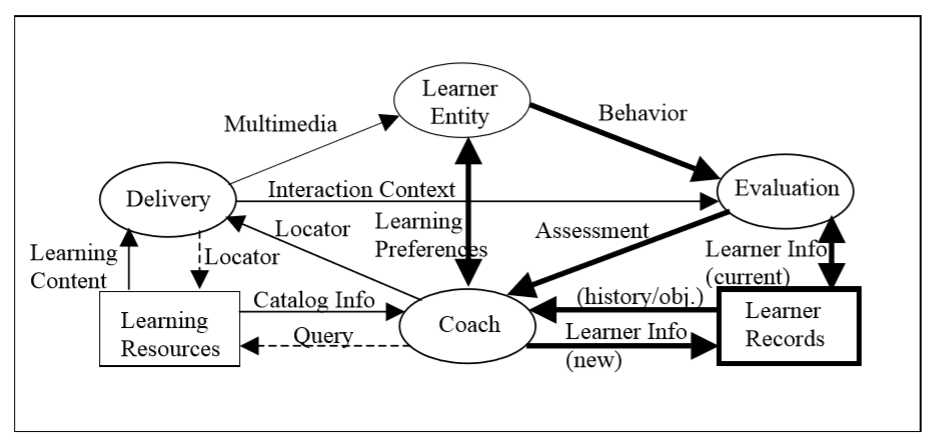
\includegraphics[width=1.0\textwidth]{LTSA}
    \caption[Learning Technology Systems Architecture]
        {Learning Technology Systems Architecture, IEEE P1484.1/D9 \citep{farance1999learning}}
    \label{fig:LTSA}
\end{figure}

E-learning has been growing as an industry and research area, and various standards have been devised. One of the most
useful is IEEE P1484.1/D9: the Learning Technology Systems Architecture (LTSA). It provides a valuable way of organising 
the scope and discussion around proposed e-Learning systems, identifying four main components: learner entity, coach, 
delivery and evaluation; and two main resources: learning resources and learner records (See figure \ref{fig:LTSA}).

Identifying what a future, blockchain based system could improve in these critical areas 
can further enhance this project. \citet{garrison2011learning} identified several areas 
that current e-Learning research and practices focus on:

\begin{itemize}
    \item Enhancing the learning community and social presence
    \item Enhancing the cognitive (practical inquiry and critical thinking) presence, 
    especially with asynchronous (pre-recorded)
    \item Self-regulation and motivation: a self-regulated learner achieves more
    \item 
\end{itemize}

\subsection{Self-Regulation and Motivation}

There are several dimensions of self-regulation that will help a learner stay on an 
e-Learning course or curriculum:

\begin{table}[!ht] 
    \caption{Self-Regulation and Motivation Strategies, adapted from \citep[p.189]{o2013web}}
    \centering
    \label{table:Self-regulation Dimensions}
    \begin{tabular}{l c }
        \toprule
        Self-regulation Dimensions & Examples of Motivation Strategies \\ 
        \midrule
        Motives & Setting challenging but achievable goals \\ \hline
        Methods of Learning & Summarisation, outline-formatted notes, \\
        & interrogation and rehearsal, etc\\ \hline
        Time Management & Prioritizing tasks, dealing with procrastination\\ \hline
        Physical Environment & An environment conducive to learning\\ \hline
        Social environment & Help seeking: knowing when help is needed,\\
        & identifying sources of help, framing help request,\\
        & evaluating help received\\ \hline
        Performance & Observing and reflecting upon performance\\
        & with short-term and long-term goals\\
        \bottomrule
    \end{tabular}
\end{table}

An e-learning programme should equip a learner with these self-regulation skills,
and the e-learning system should provide tools that facilitate and enable the 
motivation strategies.

\subsection{Security and Privacy}

The security of e-learning systems have also been a concern. For example, \citet{el2003privacy} noted that “While many 
advances have been made in the mechanics of providing online instruction, the needs for privacy and security have to-date 
been largely ignored. At best they have been accommodated in an ad-hoc, patchwork fashion.” 

\section{Properties of Blockchain Technologies}

Impossible to collude: executed by transparent code, increase trust and enables reputation building for even new entrants to 
the education market
Protects learner: guaranteed records and rewards
% Scam? Reputation building? https://books.google.co.uk/books?id=jEsRVTbukyMC&lpg=PR5&ots=DKQbVRC8Yh&dq=high%20education%20assessment%20reputation&lr&pg=PA233#v=onepage&q=high%20education%20assessment%20reputation&f=false
Administration costs of higher education
Smart Contract: secure and cutting the middleman

Characteristics of a blockchain ledger such as Hyperledger:
1. Shared Ledger: 
shared across education and government authorities
2. Smart Contract: 
Swan (2015, p.62) proposed that “rules embedded in learning smart contracts could automatically confirm the completion of learning modules 
through standardized online tests”.
3. Privacy: 
a. Appropriate Visibility
b. Transactions are secure, authenticated and verifiable
4. Consensus: All shared ledger parties agree to transactions

Openness and transparency of online courses and online assessments is encouraged: using an interpreted language, instead of a compiled 
one, to write the smart contract, so the actual code is visible on the blockchain and can be easily inspected
% Trust in Education Providers can be maintained the identity of any addition or modification to the record can be traced, records cannot 
be removed or altered
% Privacy of course participants is protected: events are publicly-accessible, but not publicly readable without a digital key
Resilient to loss of infrastructure: records are distributed over a network of participating computers

\section{Existing Efforts in Blockchain for Education}

% chapter 1
% The potential of blockchain enabled systems in education has been noted by the community, with \citet[p.62]{swan2015blockchain} 
% proposing that “learning smart contracts could automatically confirm the completion of learning modules through standardized 
% online tests”. Appropriate configurations in permissions and visibility can also provide improved security and privacy to e-Learning.

\subsection{Blockcerts}

A current blockchain in education use case: Blockcerts
Blockcerts is an MIT backed open standard for blockchain certificates. Education providers can use it to store the records of 
certifications they have awarded, in a way where they are immutable and decentralised. 

\subsection{OpenLearn}


% Uncomment this line, when you have siunitx package loaded.
%The SI Units for dynamic viscosity is \si{\newton\second\per\metre\squared}.
% I'm going to randomly include a picture Figure~\ref{fig:minion}.


% If you have trouble viewing this document contact Krishna at: \href{mailto:kks32@cam.ac.uk}{kks32@cam.ac.uk} or raise an issue at \url{https://github.com/kks32/phd-thesis-template/}


% \begin{figure}[htbp!] 
% \centering    
% 
\includegraphics[width=1.0\textwidth]{minion}
% \caption[Minion]{This is just a long figure caption for the minion in Despicable Me from Pixar}
% \label{fig:minion}
% \end{figure}


% \section*{Enumeration}
% Lorem ipsum dolor sit amet, consectetur adipiscing elit. Sed vitae laoreet lectus. Donec lacus quam, malesuada ut erat vel, consectetur eleifend tellus. Aliquam non feugiat lacus. Interdum et malesuada fames ac ante ipsum primis in faucibus. Quisque a dolor sit amet dui malesuada malesuada id ac metus. Phasellus posuere egestas mauris, sed porta arcu vulputate ut. Donec arcu erat, ultrices et nisl ut, ultricies facilisis urna. Quisque iaculis, lorem non maximus pretium, dui eros auctor quam, sed sodales libero felis vel orci. Aliquam neque nunc, elementum id accumsan eu, varius eu enim. Aliquam blandit ante et ligula tempor pharetra. Donec molestie porttitor commodo. Integer rutrum turpis ac erat tristique cursus. Sed venenatis urna vel tempus venenatis. Nam eu rhoncus eros, et condimentum elit. Quisque risus turpis, aliquam eget euismod id, gravida in odio. Nunc elementum nibh risus, ut faucibus mauris molestie eu.
%  Vivamus quis nunc nec nisl vulputate fringilla. Duis tempus libero ac justo laoreet tincidunt. Fusce sagittis gravida magna, pharetra venenatis mauris semper at. Nullam eleifend felis a elementum sagittis. In vel turpis eu metus euismod tempus eget sit amet tortor. Donec eu rhoncus libero, quis iaculis lectus. Aliquam erat volutpat. Proin id ullamcorper tortor. Fusce vestibulum a enim non volutpat. Nam ut interdum nulla. Proin lacinia felis malesuada arcu aliquet fringilla. Aliquam condimentum, tellus eget maximus porttitor, quam sem luctus massa, eu fermentum arcu diam ac massa. Praesent ut quam id leo molestie rhoncus. Praesent nec odio eget turpis bibendum eleifend non sit amet mi. Curabitur placerat finibus velit, eu ultricies risus imperdiet ut. Suspendisse lorem orci, luctus porta eros a, commodo maximus nisi.

% Nunc et dolor diam. Phasellus eu justo vitae diam vehicula tristique. Vestibulum vulputate cursus turpis nec commodo. Etiam elementum sit amet erat et pellentesque. In eu augue sed tortor mollis tincidunt. Mauris eros dui, sagittis vestibulum vestibulum vitae, molestie a velit. Donec non felis ut velit aliquam convallis sit amet sit amet velit. Aliquam vulputate, elit in lacinia lacinia, odio lacus consectetur quam, sit amet facilisis mi justo id magna. Curabitur aliquet pulvinar eros. Cras metus enim, tristique ut magna a, interdum egestas nibh. Aenean lorem odio, varius a sollicitudin non, cursus a odio. Vestibulum ante ipsum primis in faucibus orci luctus et ultrices posuere cubilia Curae; 
% \begin{enumerate}
% \item The first topic is dull
% \item The second topic is duller
% \begin{enumerate}
% \item The first subtopic is silly
% \item The second subtopic is stupid
% \end{enumerate}
% \item The third topic is the dullest
% \end{enumerate}
% Morbi bibendum est aliquam, hendrerit dolor ac, pretium sem. Nunc molestie, dui in euismod finibus, nunc enim viverra enim, eu mattis mi metus id libero. Cras sed accumsan justo, ut volutpat ipsum. Nam faucibus auctor molestie. Morbi sit amet eros a justo pretium aliquet. Maecenas tempor risus sit amet tincidunt tincidunt. Curabitur dapibus gravida gravida. Vivamus porta ullamcorper nisi eu molestie. Ut pretium nisl eu facilisis tempor. Nulla rutrum tincidunt justo, id placerat lacus laoreet et. Sed cursus lobortis vehicula. Donec sed tortor et est cursus pellentesque sit amet sed velit. Proin efficitur posuere felis, porta auctor nunc. Etiam non porta risus. Pellentesque lacinia eros at ante iaculis, sed aliquet ipsum volutpat. Suspendisse potenti.

% Ut ultrices lectus sed sagittis varius. Nulla facilisi. Nullam tortor sem, placerat nec condimentum eu, tristique eget ex. Nullam pretium tellus ut nibh accumsan elementum. Aliquam posuere gravida tellus, id imperdiet nulla rutrum imperdiet. Nulla pretium ullamcorper quam, non iaculis orci consectetur eget. Curabitur non laoreet nisl. Maecenas lacinia, lorem vel tincidunt cursus, odio lorem aliquet est, gravida auctor arcu urna id enim. Morbi accumsan bibendum ipsum, ut maximus dui placerat vitae. Nullam pretium ac tortor nec venenatis. Nunc non aliquet neque. 

% \section*{Itemize}
% \begin{itemize}
% \item The first topic is dull
% \item The second topic is duller
% \begin{itemize}
% \item The first subtopic is silly
% \item The second subtopic is stupid
% \end{itemize}
% \item The third topic is the dullest
% \end{itemize}

% \section*{Description}
% \begin{description}
% \item[The first topic] is dull
% \item[The second topic] is duller
% \begin{description}
% \item[The first subtopic] is silly
% \item[The second subtopic] is stupid
% \end{description}
% \item[The third topic] is the dullest
% \end{description}


% \clearpage

% \tochide\section{Hidden section}
% \textbf{Lorem ipsum dolor sit amet}, \textit{consectetur adipiscing elit}. In magna nisi, aliquam id blandit id, congue ac est. Fusce porta consequat leo. Proin feugiat at felis vel consectetur. Ut tempus ipsum sit amet congue posuere. Nulla varius rutrum quam. Donec sed purus luctus, faucibus velit id, ultrices sapien. Cras diam purus, tincidunt eget tristique ut, egestas quis nulla. Curabitur vel iaculis lectus. Nunc nulla urna, ultrices et eleifend in, accumsan ut erat. In ut ante leo. Aenean a lacinia nisl, sit amet ullamcorper dolor. Maecenas blandit, tortor ut scelerisque congue, velit diam volutpat metus, sed vestibulum eros justo ut nulla. Etiam nec ipsum non enim luctus porta in in massa. Cras arcu urna, malesuada ut tellus ut, pellentesque mollis risus.Morbi vel tortor imperdiet arcu auctor mattis sit amet eu nisi. Nulla gravida urna vel nisl egestas varius. Aliquam posuere ante quis malesuada dignissim. Mauris ultrices tristique eros, a dignissim nisl iaculis nec. Praesent dapibus tincidunt mauris nec tempor. Curabitur et consequat nisi. Quisque viverra egestas risus, ut sodales enim blandit at. Mauris quis odio nulla. Cras euismod turpis magna, in facilisis diam congue non. Mauris faucibus nisl a orci dictum, et tempus mi cursus.

% Etiam elementum tristique lacus, sit amet eleifend nibh eleifend sed \footnote{My footnote goes blah blah blah! \dots}. Maecenas dapibu augue ut urna malesuada, non tempor nibh mollis. Donec sed sem sollicitudin, convallis velit aliquam, tincidunt diam. In eu venenatis lorem. Aliquam non augue porttitor tellus faucibus porta et nec ante. Proin sodales, libero vitae commodo sodales, dolor nisi cursus magna, non tincidunt ipsum nibh eget purus. Nam rutrum tincidunt arcu, tincidunt vulputate mi sagittis id. Proin et nisi nec orci tincidunt auctor et porta elit. Praesent eu dolor ac magna cursus euismod. Integer non dictum nunc.


% \begin{landscape}

% \section*{Subplots}
% I can cite Wall-E (see Fig.~\ref{fig:WallE}) and Minions in despicable me (Fig.~\ref{fig:Minnion}) or I can cite the whole figure as Fig.~\ref{fig:animations}


% \begin{figure}
%   \centering
%   \begin{subfigure}[b]{0.3\textwidth}
%     
\includegraphics[width=\textwidth]{TomandJerry}
%     \caption{Tom and Jerry}
%     \label{fig:TomJerry}   
%   \end{subfigure}             
%   \begin{subfigure}[b]{0.3\textwidth}
%     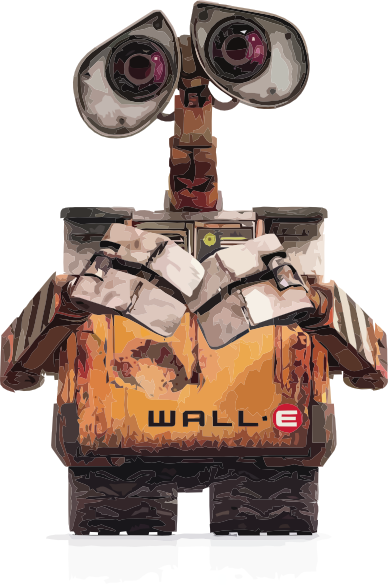
\includegraphics[width=\textwidth]{WallE}
%     \caption{Wall-E}
%     \label{fig:WallE}
%   \end{subfigure}             
%   \begin{subfigure}[b]{0.3\textwidth}
%     
\includegraphics[width=\textwidth]{minion}
%     \caption{Minions}
%     \label{fig:Minnion}
%   \end{subfigure}
%   \caption{Best Animations}
%   \label{fig:animations}
% \end{figure}


% \end{landscape}

%!TEX root = ../thesis.tex
%*******************************************************************************
%****************************** Third Chapter **********************************
%*******************************************************************************
\chapter{Approach}

% **************************** Define Graphics Path **************************
% \ifpdf
%     \graphicspath{{Chapter3/Figs/Raster/}{Chapter3/Figs/PDF/}{Chapter3/Figs/}}
% \else
%     \graphicspath{{Chapter3/Figs/Vector/}{Chapter3/Figs/}}
% \fi

\section{Agile Project Management}
\section{Software Development and Testing}
%!TEX root = ../thesis.tex
%*******************************************************************************
%****************************** Third Chapter **********************************
%*******************************************************************************
\chapter{Requirements Elicitation}
\graphicspath{{Chapter4/Figs/Raster/}{Chapter4/Figs/}}

Background literature review in Chapter 2.1 and 2.2 has driven the direction of the project and 
provided many of the functional requirements. This chapter describes the further collection of primary 
data, and provides the list of formal user requirements.

\section{Primary Data and Analysis}
Collecting primary data from shareholders of higher education e-learning systems would be able to:
\begin{itemize}
    \item reaffirm and further develop requirements obtained from literature
    \item obtain further requirements from real world painpoints and goals
\end{itemize}

\subsection{Methodology}

[TODO]

Method: qualitative

Instrument: Why interviews?

Sample: Participants are needed who are 
\begin{itemize}
    \item Teaching staff in higher education with 10+ years of experience
    \item Student
\end{itemize}Teachers with  in Who are they? Why? Convenience Sampling. Limitation: all CS department.

An ethics submission was completed on BREO and approval granted on 21st November. 
See Appendix (TODO) for the approved participant information sheet, consent form and example questions.

A total of five interviews were conducted between December 2017 and February 2018: 
two with teaching staff and three with student representatives. See table 
\ref{table:participants-req} for a more detailed description of these participants.

\begin{table}[!h] 
    \caption{Participants in primary data collection interviews}
    \centering
    \label{table:participants-req}
    \begin{tabularx}{\textwidth}{>{\bfseries}lX}
        Participant & Characterisation\\
        \toprule
        Educator A & lecturer in higher education for over 20 years, and an experienced higher education 
        administrator\\\midrule
        Educator B & lecturer in higher education for over 20 years, with research interests 
        in e-learning interactions, effectiveness and acceptance\\\midrule
        Student C & a university course representative for 3 years, which involves collecting and 
        communicating student feedback and attending staff-student liaison meetings \\\midrule
        Student D & a university peer assisted learning leader for 2 years, helping out lower level 
        students with their academic work by facilitating peer discussions, and escalating common problems
        to academic staff in debrief sessions\\\midrule
        Student E & a university course representative for 2 years and a peer assisted learning leader 
        for 1 year\\\bottomrule
    \end{tabularx}
\end{table}

\subsection{Interview Results and Analysis}

The raw data from interviews (transcripts) were contextually analysed and grouped into problem statements (PS), 
these problem statements were then sorted into groups to produce an affinity diagram (See figure 
\ref{fig:ps-affinity}).

Below you will find the sample questions asked for each group, detailed descriptions and relevant transcript 
snippets for each problem statements. 
Any specifics regarding course, staff and event details have been anonymised.

\begin{figure}[!ht] 
    \centering    
    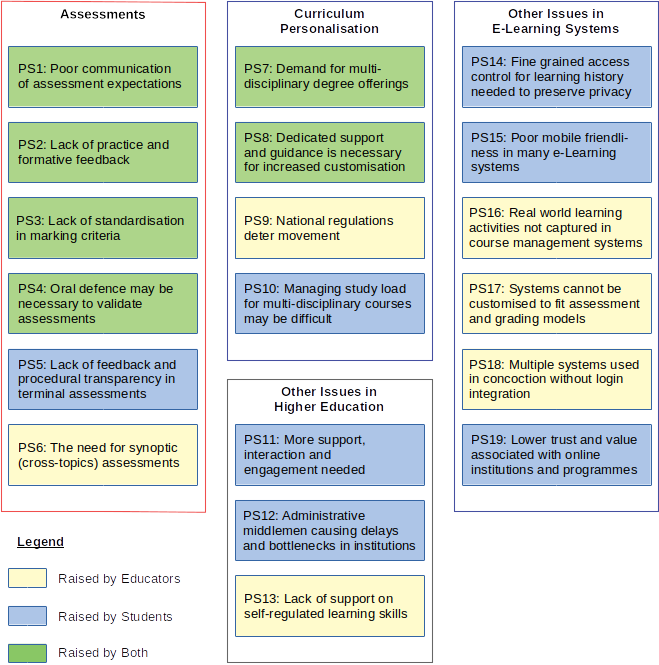
\includegraphics[width=1.0\textwidth]{ps-affinity}
    \caption[Affinity diagram for primary data]
        {Affinity diagram for problem statements devised from primary data}
    \label{fig:ps-affinity}
\end{figure}



\section{Formal Requirements}

Table \ref{table:fx-reqs} lists out the functional requirements (FR) adopted by this 
project going forward. They are related to one or more of the problem statements (PS) gathered 
above from primary data, or to the literature reviewed in Chapter 2. 

Table \ref{table:nonfx-reqs} lists the non-functional requirements (NR) adopted by this 
project going forward. They are related to one or more of the problem statements (PS) gathered, 
or to usability heuristics.

These requirements have been ranked with the MoSCoW prioritisation
framework, which specified four levels of priority: Must Have, Should Have, Could Have, and Won’t Have 
this time \citep{agile2018moscow}. The MoSCoW levels are given from mainly a system engineering perspective 
in planning the minimum viable product for the demonstrator of this project, 
and do not necessarily reflect the priorities of the stakeholders.

\begin{table}[!h] 
    \caption{Prioritised list of functional requirements for this project}
    \centering
    \label{table:fx-reqs}
    \begin{tabularx}{\textwidth}{>{\bfseries}l>{\hsize=1.5\hsize}X>{\hsize=.5\hsize}Xl}
        & Requirement Statements & Related To & MoSCoW\\
        \toprule
        FR1 & The system would store learner records on a blockchain 
        & Ch 2.2.1 (LTSA) & Must Have
        \\\midrule
        FR2 & Teachers would be able to create and edit learning resources
        & Ch 2.2.1 (LTSA) & Must Have
        \\\midrule
        FR3 & Teachers would be able to create and edit assessments
        & Ch 2.2.1 (LTSA) & Must Have
        \\\midrule
        FR4 & The system would enforce the provision of learning outcomes, knowledge required 
        and assessment goals at the creation or update of modules & Ch 2.1.1 (Transparency), 
        PS1 & Must Have
        \\\midrule
        FR5 & The system would enforce predefined assessments rules (eg. marking schemes, 
        transparent procedures and feedback) with smart contracts 
        & Ch 2.1.1 (Transparency), PS3, PS5 & Must Have
        \\\midrule
        FR6 & The system would allow teachers to configure multiple assessments and 
        formative assessments for modules & PS2 & Could Have
        \\\midrule
        FR7 & The system would require vivas (oral defences) after automated assessments & 
        PS4 & Could Have
        \\\midrule
        FR8 & The system would provide flexible configurability for grade schema & PS17
        & Could Have
        \\\midrule
        FR9 & Teachers would be able to create a customised list of courses 
        for a student, customising programme outcomes and specifications 
        & Ch 2.1.2 (Personalisation), PS7, PS9 & Must Have
        \\\midrule
        FR10 & The system should feature dedicated support channels between students, teachers 
        and other advisors 
        & PS8, PS11 & Should Have
        \\\midrule
        FR11 & Students would be able to add assessment submissions on the blockchain 
        & Figure \ref{fig:moocon_assess} (Concept)& Must Have
        \\\midrule
        FR12 & The system would be able to generate certificates on the blockchain when a course 
        has been completed & Figure \ref{fig:moocon_assess} (Concept) & Must Have
        \\\midrule
        FR13 & The system would allow students to control access to their education history 
        on the blockchain & PS14 & Should Have
        \\\midrule
        FR14 & The system would provide one login for content delivery, assessment and 
        record keeping & PS18 & Should Have
        \\\midrule
         &  \multicolumn{2}{c}{Requirements targetting PS6, PS10, PS13, PS16} & Won't Have
        \\\bottomrule
    \end{tabularx}
\end{table}

\begin{table}[!h] 
    \caption{Prioritised list of non-functional requirements for this project}
    \centering
    \label{table:nonfx-reqs}
    \begin{tabularx}{\textwidth}{>{\bfseries}l>{\hsize=1.6\hsize}X>{\hsize=.4\hsize}Xl}
        & Requirement Statements & Related To & MoSCoW
        \\\toprule
        NR1 & The client applications would have the same functionalities across devices and 
        a responsive interface & PS15 & Should Have
        \\\midrule
        NR2 & The client applications would fail safely and is error-forgiving 
        towards the user &  & Should Have
        \\\midrule
        NR3 & The client applications would notify users of relevant events on the blockchain
        network &  & Should Have
        \\\midrule
        NR4 & The system should be able to reduce administrative work & PS12 & Should Have
        \\\midrule
        NR5 & The system should be able to create more trust in online education providers 
        and programmes & PS19 & Should Have
        \\\bottomrule
    \end{tabularx}
\end{table}
%!TEX root = ../thesis.tex
%*******************************************************************************
%****************************** Third Chapter **********************************
%*******************************************************************************
\chapter{Design}

\section{Choice of Blockchain Development Ecosystem}

\section{Participants, Assets and Transactions in the Blockchain Network}
And now I begin my third chapter here \dots

\subsection{Access and Permissions on Assets}

\section{Logic and Events in Smart Contracts}

\section{User Interfaces for Client Applications}
%!TEX root = ../thesis.tex
%*******************************************************************************
%****************************** Sixth Chapter **********************************
%*******************************************************************************
\chapter{Implementation}

\graphicspath{{Chapter6/Figs/Raster/}{Chapter6/Figs/}}

\section{Development Environment and Tools}

Specific systems and tools were used to build the demonstrator network and client applications (as in Figure \ref{fig:platform_stats}).
These choices and their rationale are detailed below:

\begin{figure}[!ht]
	\centering
	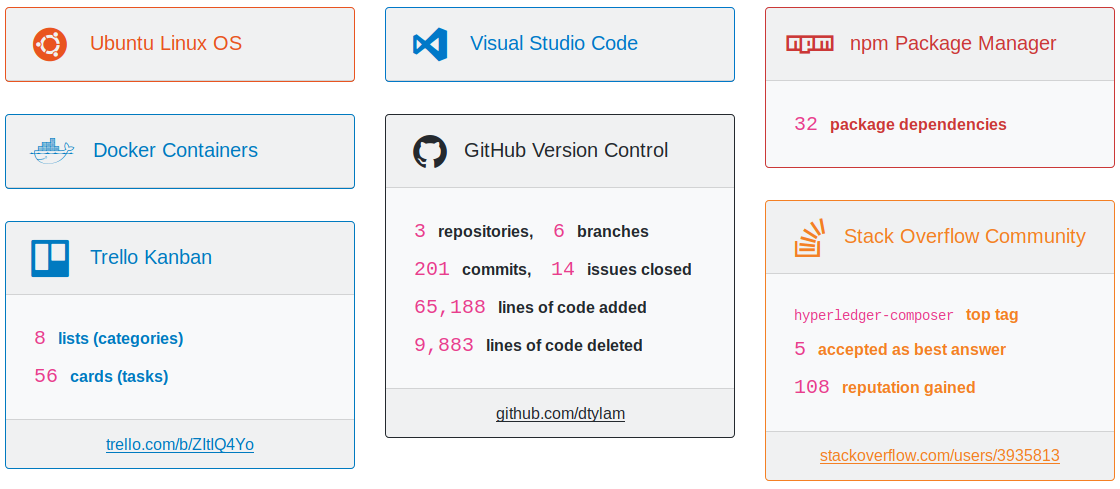
\includegraphics[width=1.0\textwidth]{platform_stats}
	\caption[Development Tools and Usage Statistics]
	{A visual overview of the tools used and their usage statistics (Last Updated: 26th Mar 2018))}
	\label{fig:platform_stats}
\end{figure}

\underline{Operating System}: The developer's guide for both Hyperledger Composer and Hyperledger Fabric
recommends using Ubuntu or Mac OS as the host operating system for development.
Ubuntu is selected for being the free and open source option. The development personal computer, which was originally
a Windows machine, was set up to dual boot with the latest Ubuntu release.

\underline{Version Control}: A version control system or software keeps track of source code modifications,
so that developers can compare earlier versions of the code, revert changes, and
minimise disruptions of mistakes \citep{atlassian2018vcs}. It is essential to medium to large scaled projects.

All work done at the implementation stage was tracked with the version control system Git.
Git is a distributed version control system, where repositories can be backed up to a remote server,
such as on the cloud. This is done with GitHub, a git-based version control, code hosting and
project management service that offers free private repositories to verified students \citep{github2018education}.

\underline{Code Editor}: The Hyperledger Composer framework does not require a dedicated integrated
development environment and recommends using a text editor. Visual Studio Code, an open source text editor developed
by Microsoft was chosen as it has a dedicated official syntax checking and beautifying plugin for Hyperledger Composer.

\underline{Community Support}: Hyperledger Composer and Hyperledger Fabric have active communities on Stack Overflow,
a popular online community forum for developers to discuss coding problems. Throughout the duration of the project,
it has been a source of solutions to common problems faced and solved by many other users. Towards the end of the project,
answer contributions were also made.

Several other tools were also used, for example, as previously mentioned in Chapter 3, Trello was used to manage
feature prioritisation for the agile development process. The use of Docker containers, Node.js and npm 
will be explained in due course below.

\section{Architecture and Tech Stack}

\begin{figure}[!ht]
	\centering
	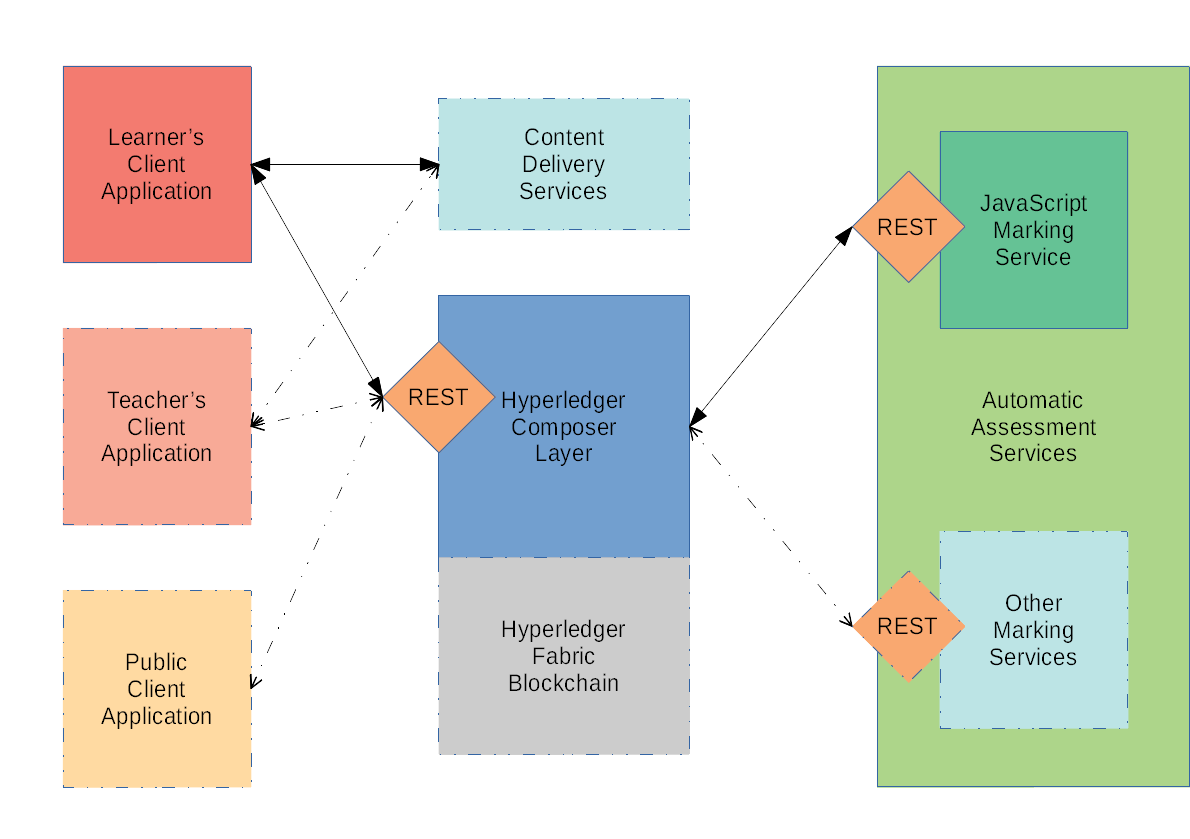
\includegraphics[width=0.9\textwidth]{architecture}
	\caption[Demonstrator Component Architecture]
	{Component architecture overview for the demonstrator system built (dashed lines components were not built)}
	\label{fig:architecture}
\end{figure}

The microservices architecture pattern is used to design the demonstrator system. Microservices is a pattern proposed by
\citet{richardson2018ms} that structures a system as a set of loosely coupled, collaborating services, partitioned so that
each service corresponds to a business capability.

In the demonstrator system (as in Figure \ref{fig:architecture}), this is exemplified by the separation of teacher and student applications,
the separation of content delivery and student records (blockchain), and the separation of different automatic marking services.
They communicate through RESTful web protocols (HTTP and JSON).
This also enables the use of different technologies, separate testing and deployment for each component.

Figure \ref{fig:techstack} shows an alternate overview of the demonstrator system with its technology stack.
These main software packages are described further below.

\begin{figure}[!ht]
	\centering
	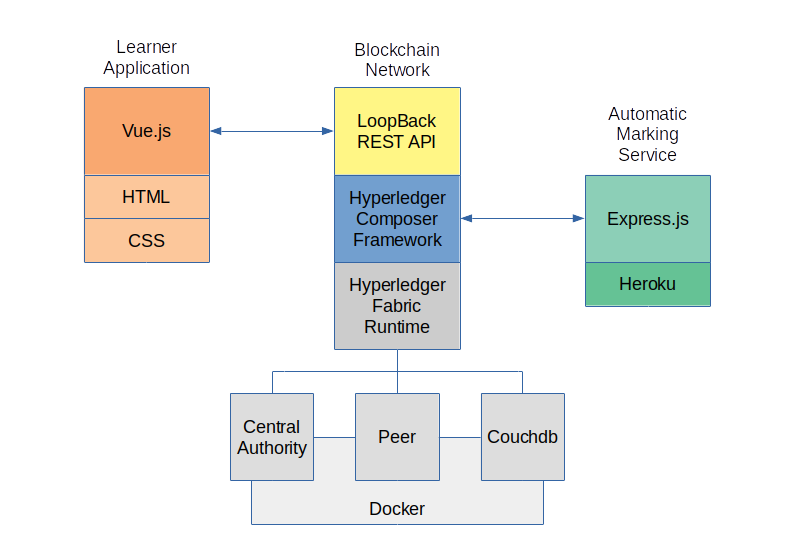
\includegraphics[width=0.85\textwidth]{techstack}
	\caption[Demonstrator Technology Stack]
	{Technology Stack overview for the demonstrator system built}
	\label{fig:techstack}
\end{figure}

\subsection{Client Applications}

The client applications for learners and teachers have to be highly dynamic (non-static) web applications,
with the JavaScript scripting language facilitating most of the user interactions.

Vue.js is a JavaScript-based framework for developing web interfaces. Vue.js was chosen over other
popular frameworks such as React.js and Angular.js because it is focused on the view layer and is much
simpler and faster to learn. The Node.js JavaScript runtime is used to run the Vue.js applications. The npm package manager
is used to install and manage the packages used. See more details such as version numbers in Appendix B.1.

\subsection{Blockchain Network}

Hyperledger Composer deploys to Hyperledger Fabric, which runs on Docker.
Docker is a containerisation platform used to develop distributed systems.
A container is a lightweight, stand-alone package of a piece of software that includes everything
needed to run it from code and tools to system settings.

Docker can emulate multiple servers and run them separately on one development machine.
This provides the peers that are needed to host the distributed ledger. 
A minimum of three docker containers are required to start a
Fabric blockchain: the Central Authority server, a minimum of one peer server, and a CouchDB server,
which is a database that stores the state of the blockchain in a queryable form.

See the full list of pre-requisites and dependencies in in Appendix B.2.

\subsection{Automatic Marking Service}

More automatic marking services were originally planned but due to time constraints only
a simple JavaScript server that checks for file equivalence was implemented.

This was written with Express.js, a minimal Node.js web application framework and hosted
on Heroku, a Node.js capable cloud platform with a free tier. See the full list of pre-requisites and dependencies in in Appendix B.3.

\section{Blockchain Network Development}

Beginning here, progress descriptions and evidence of implementation work will be presented. 
Github repository links are provided. Alternately a copy of the code is in Supporting Materials/Implementation/.

\subsection{Command Line Interface}
Using Docker, setup images of Hyperledger Fabric were downloaded, the basic three servers were set up
and a certificate for the central authority administrator was generated. This allows Hyperledger Composer
to later authenticate as the blockchain administrator and import custom network definitions.

The Hyperledger Composer notations from the design phase where packaged into
a business network archive (.bna) file, and deployed to the Hyperledger Fabric blockchain.

Three bash shell scripts were written:
\begin{enumerate}
	\setlength\itemsep{0em}
	\item \textit{start.sh}: this script starts Hyperledger Fabric, generate the minimum number of peers,
	      and connects as the blockchain administrator. It then creates the .bna file with Hyperledger Composer
	      and deploys it to the Fabric blockchain.
	      See Figure \ref{fig:startsh} for a screenshot of the script running.
	      \begin{figure}[!ht]
		      \centering
		      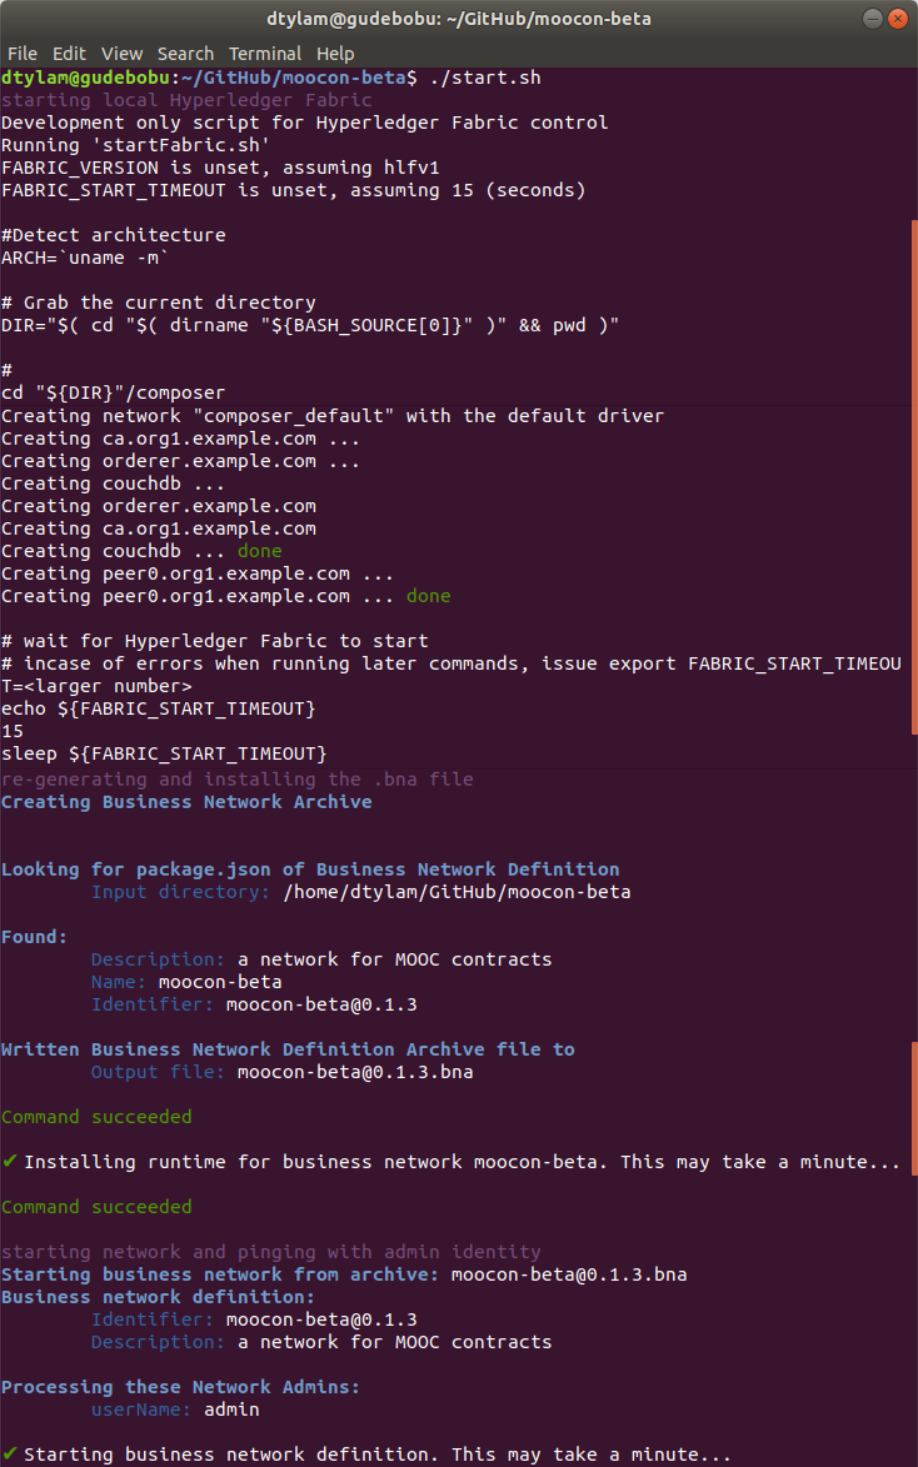
\includegraphics[width=0.85\textwidth]{startsh}
		      \caption[Blockchain Startup Script Screenshot]
		      {Screenshot of the start.sh script in action in a command line interface}
		      \label{fig:startsh}
	      \end{figure}
	\item \textit{load\_participant.sh}: this script connects as the blockchain administrator and creates
	      three \textit{Learner}, four \textit{Teacher} and two \textit{Reader} participants on the blockchain.
	      A .card file is created for each participant, which contains the certificate they need to
	      connect to the blockchain as themselves. In the final stages of development, this script is called by
	      the previous \textit{start.sh} to simplify the starting and loading process.
	      See Figure \ref{fig:load_participantsh} for a screenshot of the script running.
	      \begin{figure}[!ht]
		      \centering
		      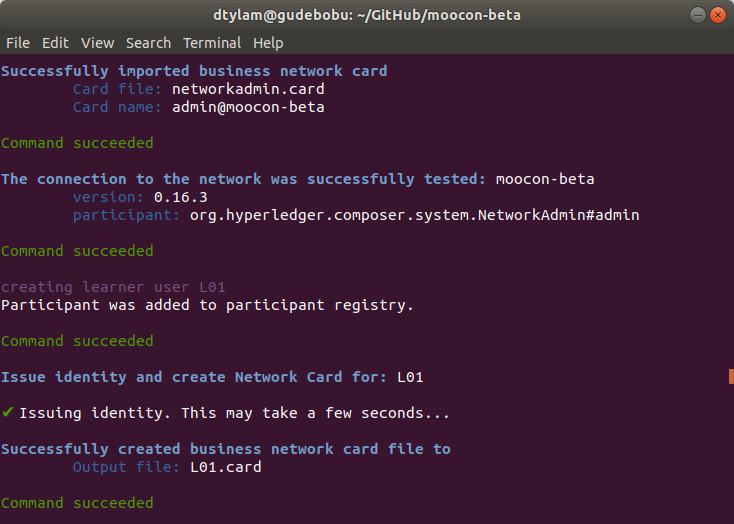
\includegraphics[width=0.85\textwidth]{load_participantsh}
		      \caption[Participant Loading Script Screenshot]
		      {Screenshot of the load\_participant.sh script in action in a command line interface}
		      \label{fig:load_participantsh}
	      \end{figure}
	\item \textit{destroy.sh}: at the end of every development session, the blockchain is completely
	      erased and removed. This is because unwanted data entries or transactions may have occurred, and
	      the blockchain schema can only be changed with a hard fork/ restart.
	      See Figure \ref{fig:destroysh} for a screenshot of the script running.
	      \begin{figure}[!ht]
		      \centering
		      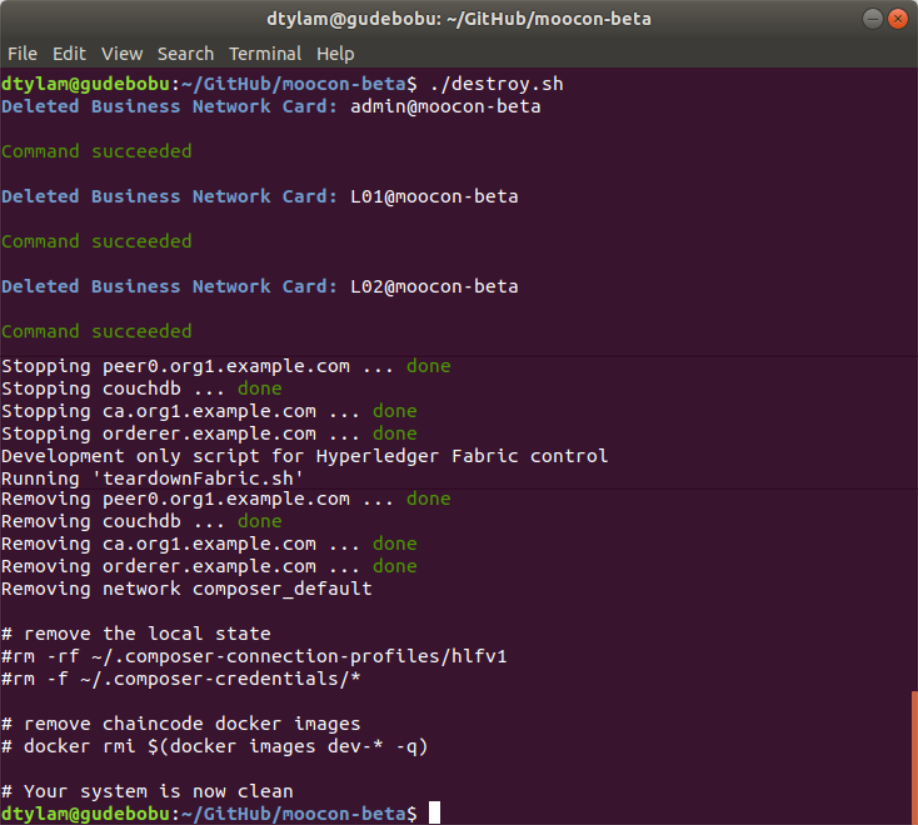
\includegraphics[width=0.85\textwidth]{destroysh}
		      \caption[Blockchain Teardown Script Screenshot]
		      {Screenshot of the destroy.sh script in action in a command line interface}
		      \label{fig:destroysh}
	      \end{figure}
\end{enumerate}

The GitHub source code repository used for the blockchain schema and command line scripting
is hosted at \href{https://github.com/dtylam/moocon-beta}{\underline{github.com/dtylam/moocon-beta}}.
Three branches (significant iterations) were created for this component, below in chronological order:
\begin{enumerate}
	\setlength\itemsep{0em}
	\item \textit{moocon-alpha} branch: this is an archived repository of design work done with version 0.15.x of
	      Hyperledger Composer, the project upgraded to version 0.16 in December, which contained breaking changes.
	      The 0.16 upgrade was recommended by the Hyperledger developers because it is a long-term support
	      release that is feature complete and stable, and adds the useful .card file authentication protocol.
	\item \textit{master} branch: this is the original working branch on Hyperledger Composer 0.16, a bulk of
	      design and development work was done, and changes to the schema and transactions were made based on
	      literature review and background research.
	\item \textit{bcu} branch: this is the final, demonstration ready branch named after the proposed marketplace
	      "Blockchain University". Changes were made to satisfy new requirements obtained through primary data (interviews in Chapter 4).
\end{enumerate}

\subsection{Application Program Interface}

A readily available script connects the deployed blockchain to Loopback, an open source Node.js RESTful
Application Program Interface (API) framework. The command used is:

\begin{verbatim}
	composer-rest-server --card admin@moocon-beta --namespaces always 
	--websockets true --port 3000 --authentication true --multiuser true
\end{verbatim}

This hosts a production-ready API at \texttt{localhost:3000}, connected to the
server of the central authority administrator.
Figure \ref{fig:Loopback_explorer} shows the API explorer view generated by Loopback at \texttt{localhost:3000/explorer}.

\begin{figure}[!ht]
	\centering
	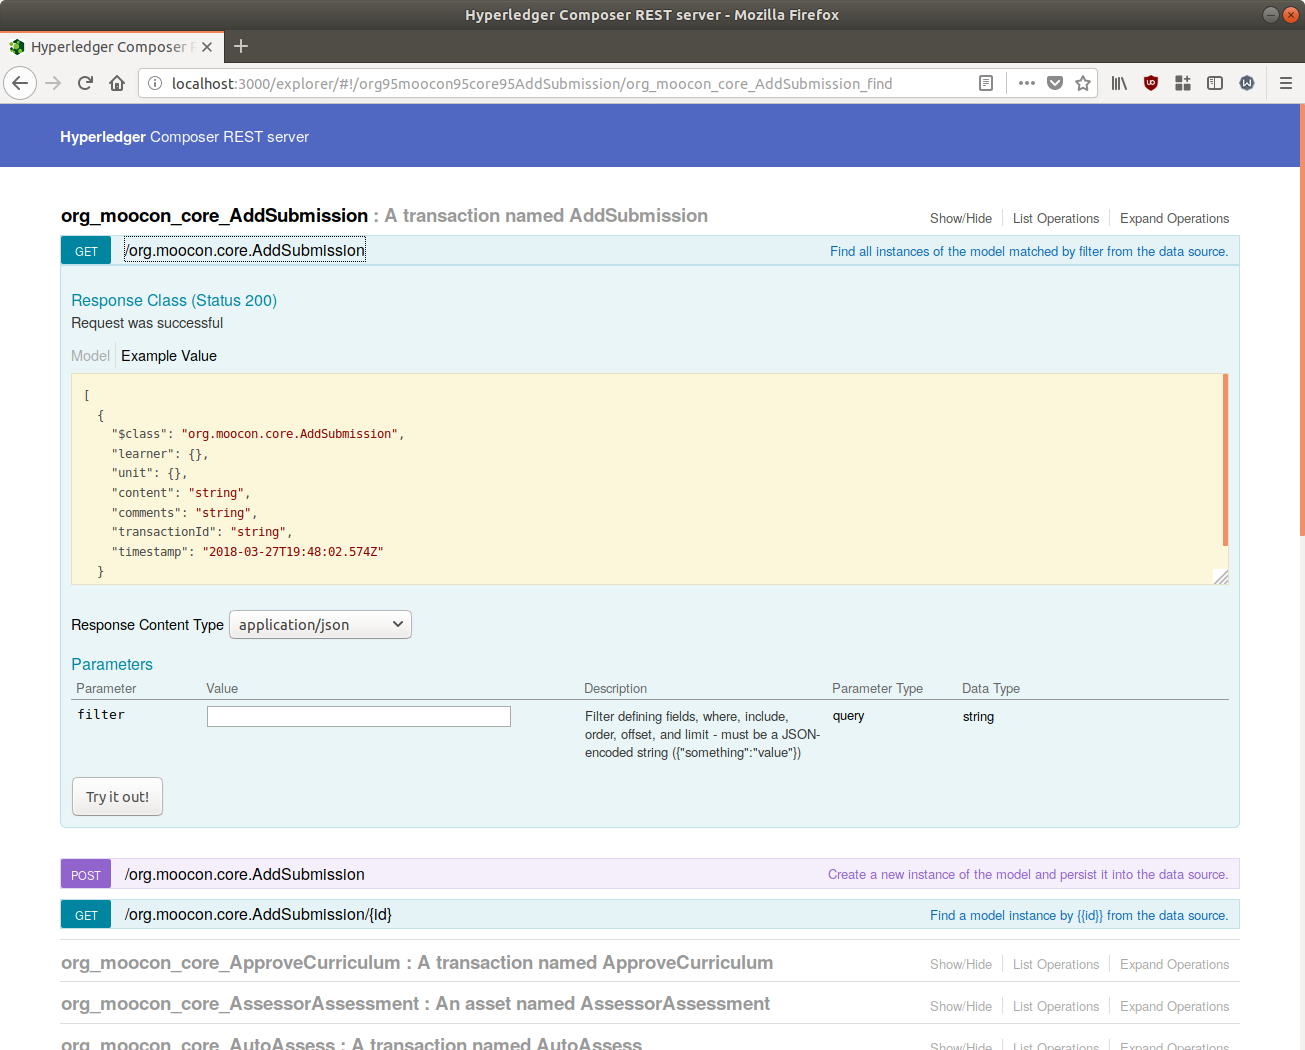
\includegraphics[width=1.0\textwidth]{Loopback_explorer}
	\caption[Hyperledger Composer Loopback REST API Screenshot]
	{Screenshot of the auto-generated Loopback Explorer for the blockchain according to Hyperledger Composer definitions}
	\label{fig:Loopback_explorer}
\end{figure}

Limitations exist for how multiple participants can use this same API. The API is authenticated as
one peer at one time. It uses a construct called \texttt{wallet} to store .card files and
switches between them to create a "multiuser" API. So to switch between users in the
client applications, a request must be made to \texttt{localhost:3000/wallet/\{cardFileName\}/setDefault}.
This limitation is accepted for the demonstrator system, as it does not impact core requirements.

Postman, a popular API testing platform, is used to run tests against the API 
before and during the development of the client applications. 
This confirms that the required API functionalities work well and 
prevents unexpected responses when building the client applications.

These tests were a form of grey-box testing. Knowledge about the API endpoints 
and parameters is required, but knowledge about how the Blockchain Network schema
and transactions work is not required. 

\clearpage
\begin{figure}[!ht]
	\centering
	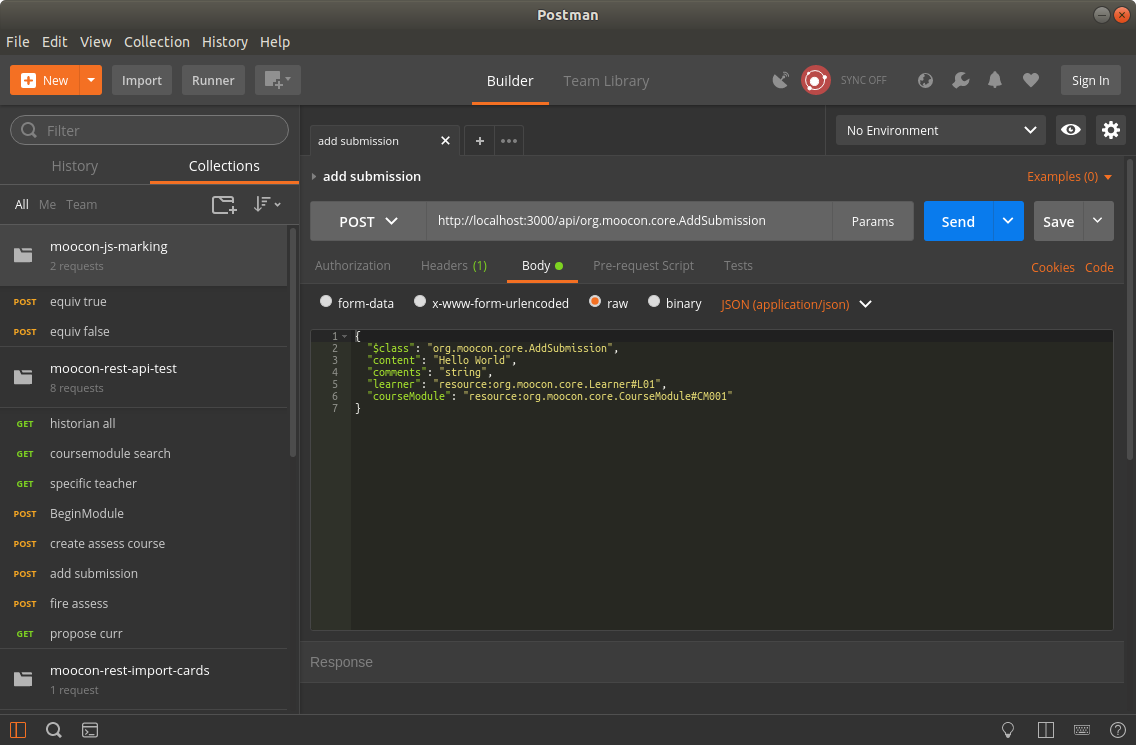
\includegraphics[width=1.0\textwidth]{postman}
	\caption[Postman API Testing Example Screenshot]
	{Postman API Testing Example Screenshot}
	\label{fig:postman}
\end{figure}

\section{Automatic Marking Service Development}

The first iteration of the Blockchain Network has no automatic marking Smart Contract features.
This is due to a limitation found during development of the original design. The original design
of the Automatic Assessment Smart Contract would have the Smart Contract run a custom block of chaincode
created by a Teacher for each assessment (See left-hand side of Figure \ref{fig:automarkinglim}).

However, the Hyperledger Composer framework does not allow chaincode to run code foreign to its main packages and vanilla JavaScript.
This is due to the transpilation and deployment of Hyperledger Composer chaincode to the Hyperledger Fabric blockchain,
a process which ordinary developers have no convenient controls over. It will not be able to accept new snippets of code,
created and uploaded to the blockchain by Teacher participants.

\begin{figure}[!ht]
	\centering
	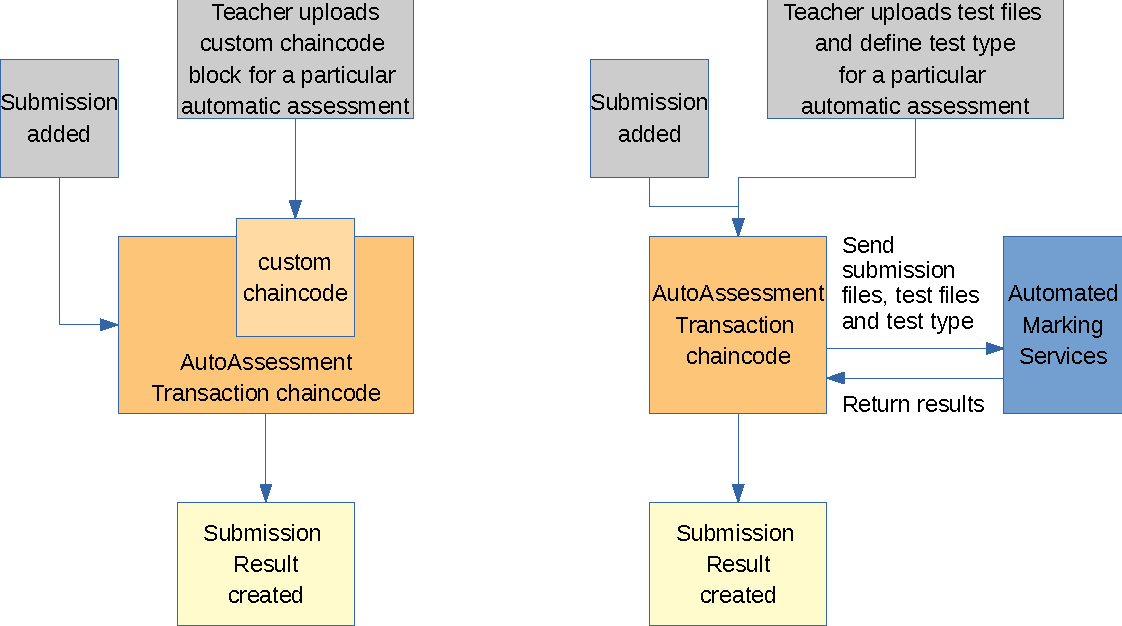
\includegraphics[width=0.9\textwidth]{automarkinglim}
	\caption[AutoAssessment Smart Contract Design Change]
	{Flowchart of the original design (left) and the technically informed design (right) of how the Automatic Assessment Smart Contract should run}
	\label{fig:automarkinglim}
\end{figure}

Understanding this limitation and after studying documentations further, a technically informed design was created
(See right-hand side of Figure \ref{fig:automarkinglim}). he Hyperledger Composer framework allows chaincode
to communicate with external APIs through a built-in method \texttt{post(url, data)} where \texttt{url} is
the endpoint address of the desired API and \texttt{data} is a blockchain asset or concept serialised into JSON format.

This limitation and subsequent redesign has actually inspired the microservices architectural approach covered in the previous section 6.1.

To use the \texttt{post(url, data)} functionality effectively, an extra asset \textit{AutoAssessRequest} was added to the blockchain schema.
\textit{AutoAssessRequest} would contain the submission content file, the test file on the blockchain for this assessment, the test type of
this assessment (eg. software testing, AI testing, etc), and an API response field. This packages all the information the external
Automated Marking Services will need, and keep the request and response records permanently on the blockchain.

To build an example automated marking service, a string equivalence test was created on a simple Express.js application server.
Here is the simple code snippet used:
\begin{verbatim}
if (req.body.testFile === req.body.content) {
    res.json(true); // if the test file is equal to the submission file
} else { res.json(false); } 
\end{verbatim}

Even though this is just a simple equivalence test, it proves the blockchain's ability to conduct automated assessments, 
and more sophisticated assessment APIs could be called or routed to.

It is essential that this testing service is available on the world-wide web, because the peers are contained in Docker
containers where the normal workstation \texttt{localhost} address is not easily reachable. Therefore, the Heroku Node.js 
hosting service is used and this example automated marking service is available at 
\href{https://moocon-js-marking.herokuapp.com/}{\underline{moocon-js-marking.herokuapp.com/}}.

The source code of this component is also tracked and hosted at 
\href{https://github.com/dtylam/moocon-js-marking}{\underline{github.com/dtylam/moocon-js-marking}}.

\section{Client Applications Development}

Before developing the client applications, some example data was created and imported into the network. 
This was nine courses modules, their module units and assessments. These data were created by loosely following 
the syllabuses of courses from Massive Open Online Courses.

A video demonstration showcasing the user journeys across both applications was created and 
available on \href{https://youtu.be/FUMBn6wPG5M}{\underline{youtube.com/FUMBn6wPG5M}}. [TODO: video too long, speed up]

An open source styling and component library, \href{https://vuematerial.io/}{Vue-material}, was used to 
create Material Design compliant user interfaces. Notes on the development process are further detailed below.

\subsection{Learner Application}

The source code of this application is tracked and hosted at 
\href{https://github.com/dtylam/moocon-learner-client}{\underline{github.com/dtylam/moocon-learner-client}}.
Two branches (significant iterations) were created for this component, below in chronological order:
\begin{enumerate}
	\setlength\itemsep{0em}
	\item \textit{master} branch: this is the first iteration made based on literature review and background research.
	\item \textit{bcu} branch: this is the final, demonstration ready branch. 
	Changes were made to satisfy new requirements obtained through primary data (interviews in Chapter 4).
\end{enumerate}

The switch from traditional static webpage development to component-driven development was a steep learning curve.
Traditional web development focuses on the separation of concerns by file types, where markup (HTML), 
styling (CSS) and scripting (JavaScript) are in different files and folders.

JavaScript-based web applications, on the other hand, encourage organisation according to functional components. 
In Vue.js for example, components (.vue) files are used to write HTML, CSS and JavaScript in one file \citep{vue2017components}, 
which creates a component in the web application. It is afterwards packaged to be production-ready with build tools.

For example, the entire web application only uses one main \texttt{index.html} page. Each main menu button 
such as "Ongoing Courses" swaps out the previous page component for another. Components can also be nested, 
the YouTube embedding view is its own component, for example.

Below are some annotated screenshots of the application (Figures \ref{fig:Learner_login} to 
\ref{fig:Learner_AC}). They attempt to showcase how requirements are fulfilled. [annotations TODO]

\begin{figure}[!ht]
	\centering
	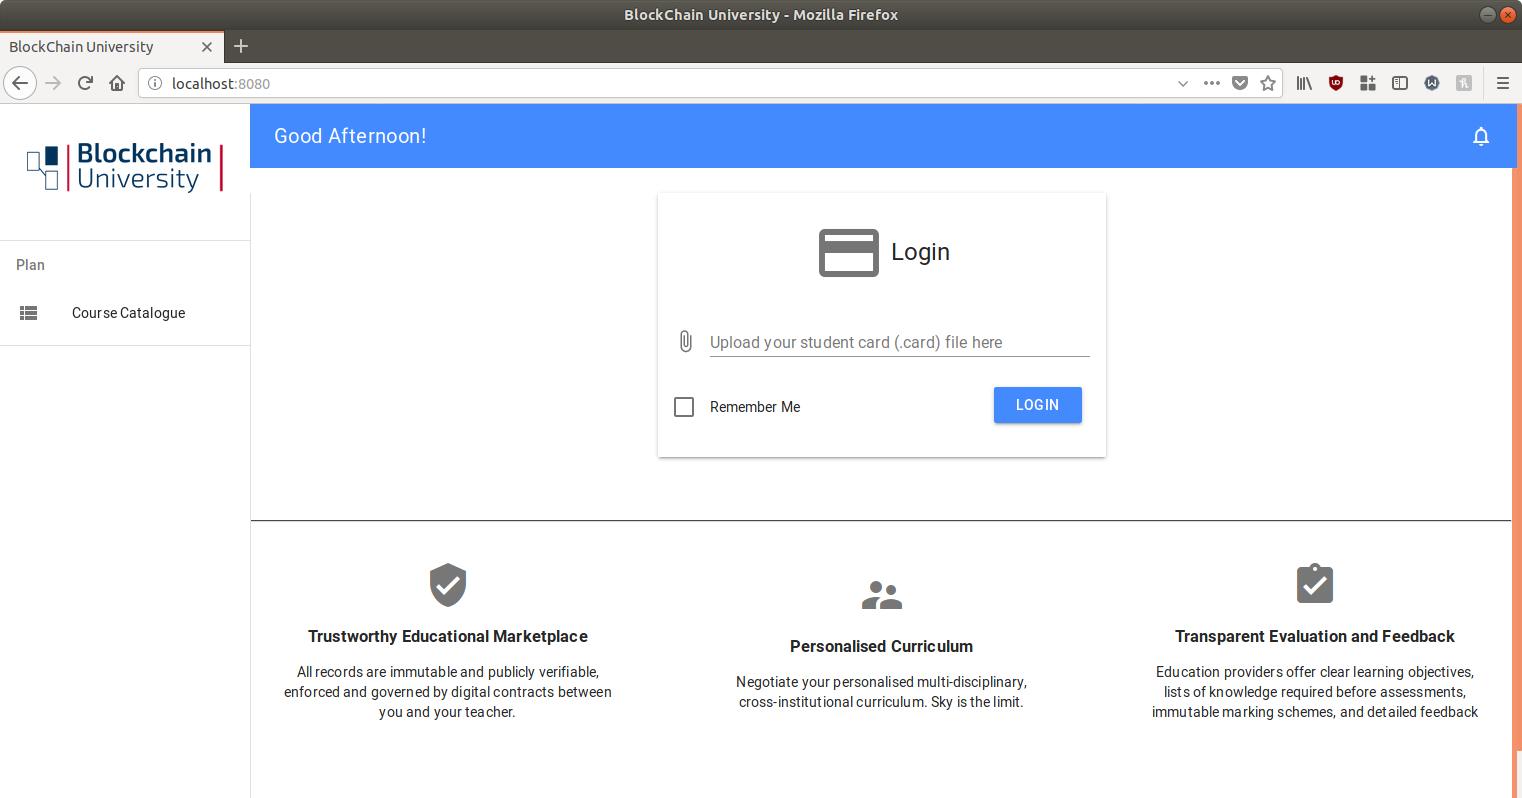
\includegraphics[width=1.0\textwidth]{Learner_login}
	\caption[Learner Application Login Page]
	{Learner Application Login Page}
	\label{fig:Learner_login}
\end{figure}

\begin{figure}[!ht]
	\centering
	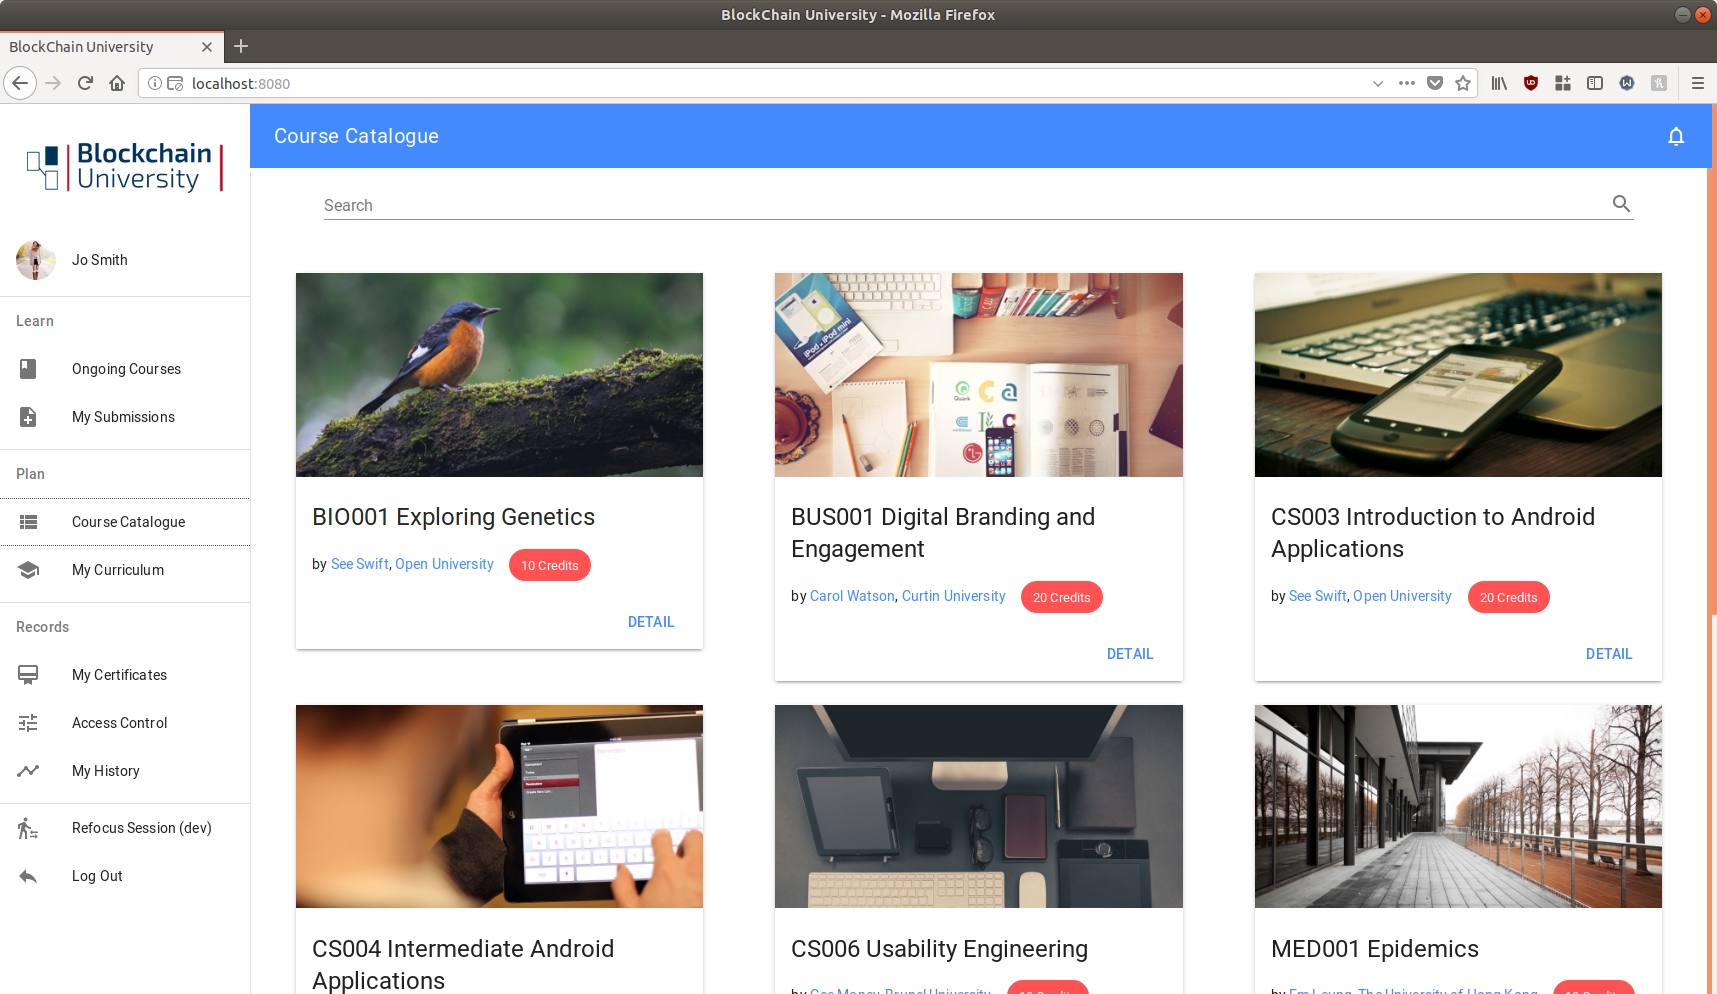
\includegraphics[width=1.0\textwidth]{Learner_allcourses}
	\caption[Learner Application Course Catalogue Page]
	{Learner Application Course Catalogue Page}
	\label{fig:Learner_allcourses}
\end{figure}

\begin{figure}[!ht]
	\centering
	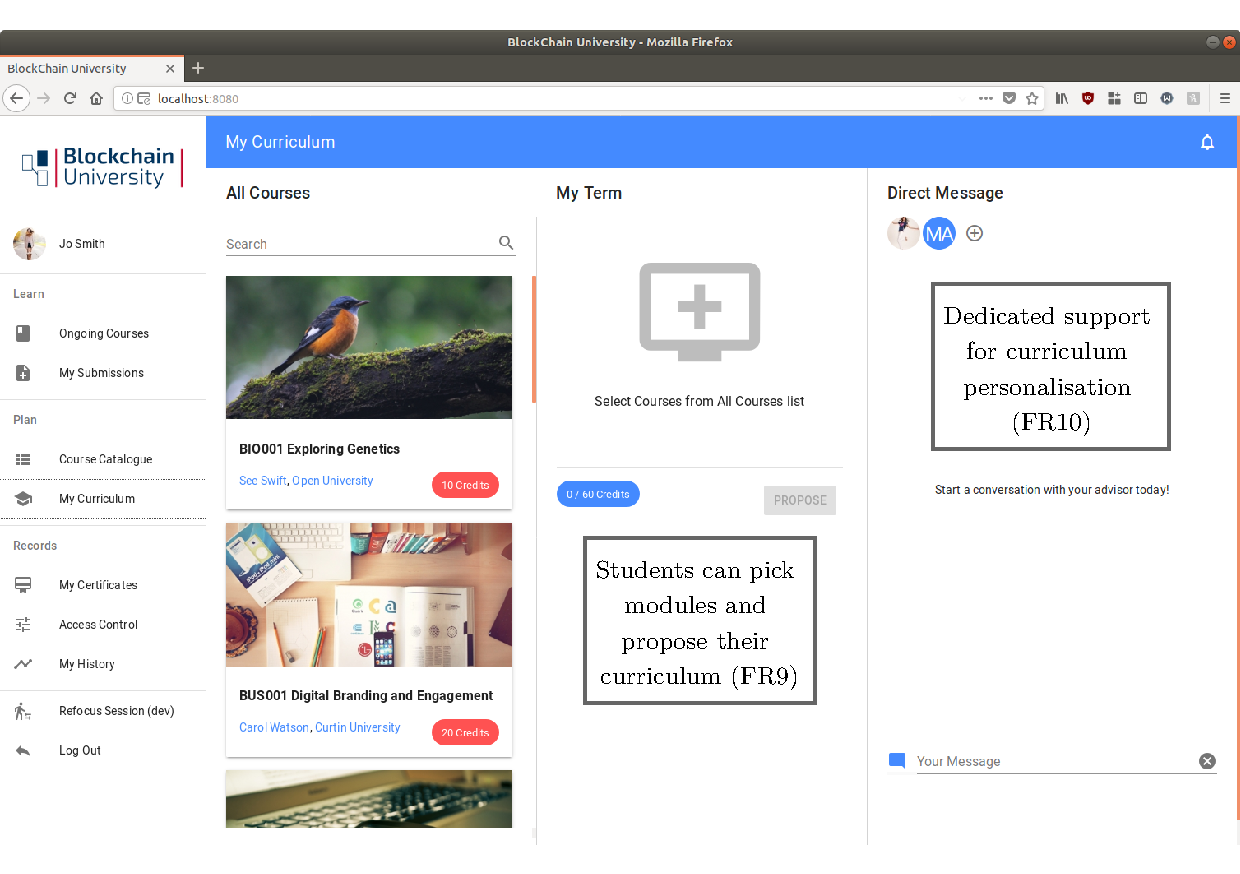
\includegraphics[width=1.0\textwidth]{Learner_customiser}
	\caption[Learner Application My Curriculum Page]
	{Learner Application My Curriculum Page}
	\label{fig:Learner_customiser}
\end{figure}

\begin{figure}[!ht]
	\centering
	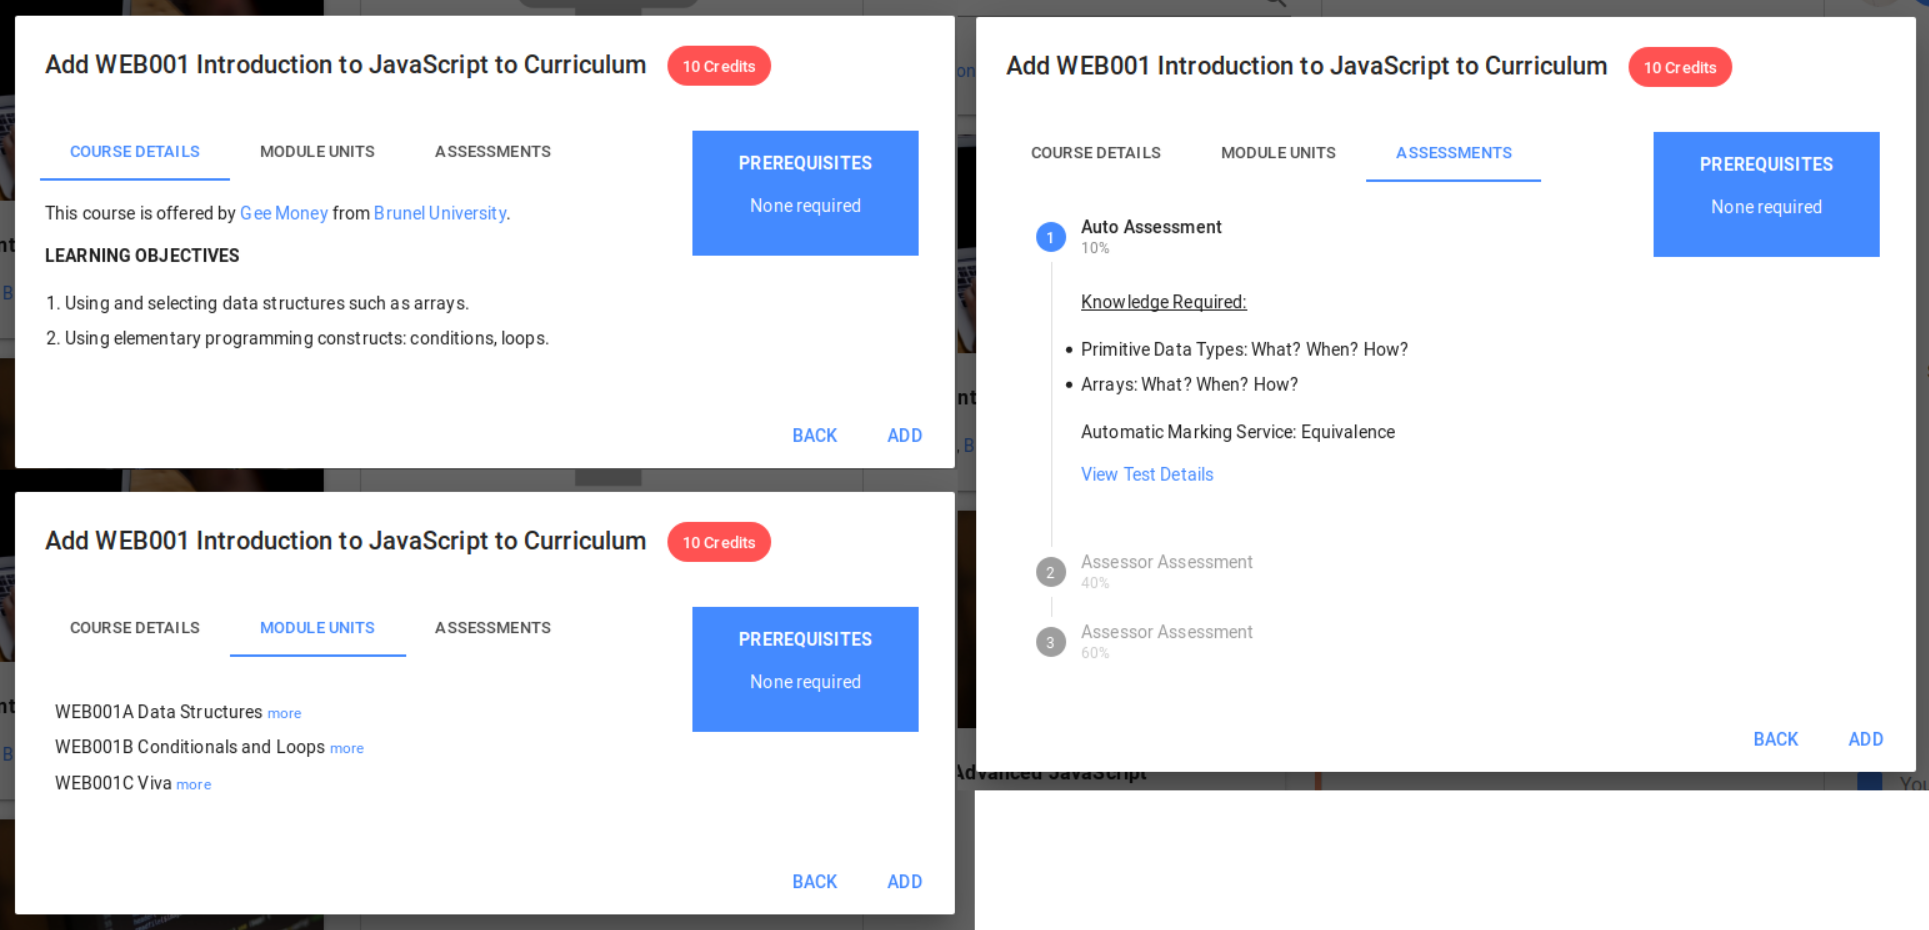
\includegraphics[width=1.0\textwidth]{Learner_cmdetails}
	\caption[Learner Application Course Module Preview Dialogue]
	{Learner Application Course Module Preview Dialogue}
	\label{fig:Learner_cmdetails}
\end{figure}

\begin{figure}[!ht]
	\centering
	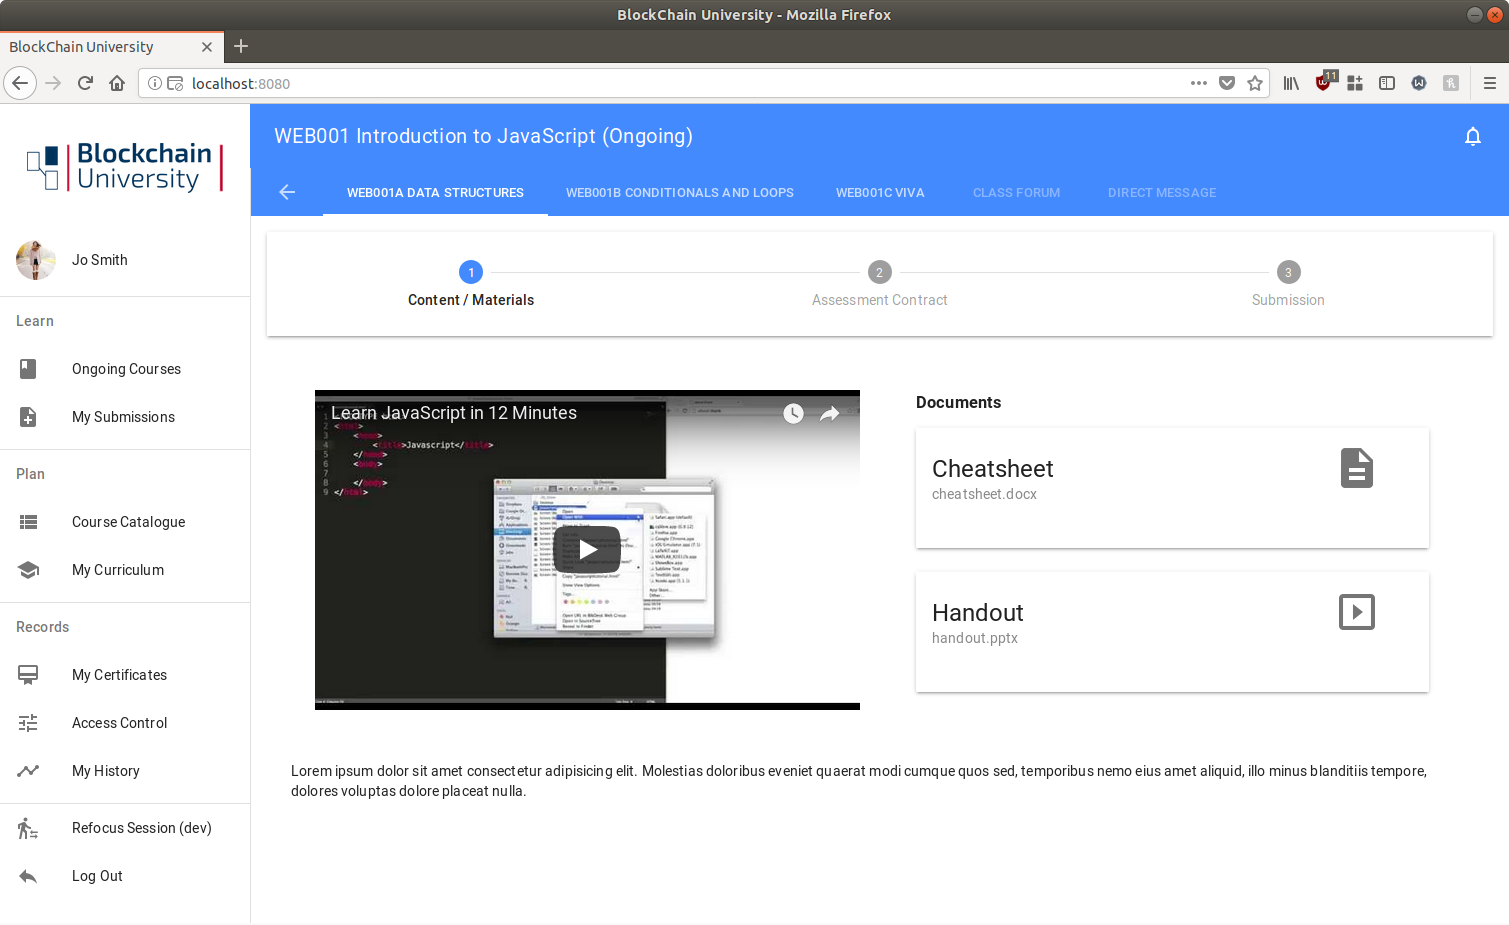
\includegraphics[width=1.0\textwidth]{Learner_ongoing1}
	\caption[Learner Application Example Ongoing Module Page]
	{Learner Application Example Ongoing Module Page}
	\label{fig:Learner_ongoing1}
\end{figure}

\begin{figure}[!ht]
	\centering
	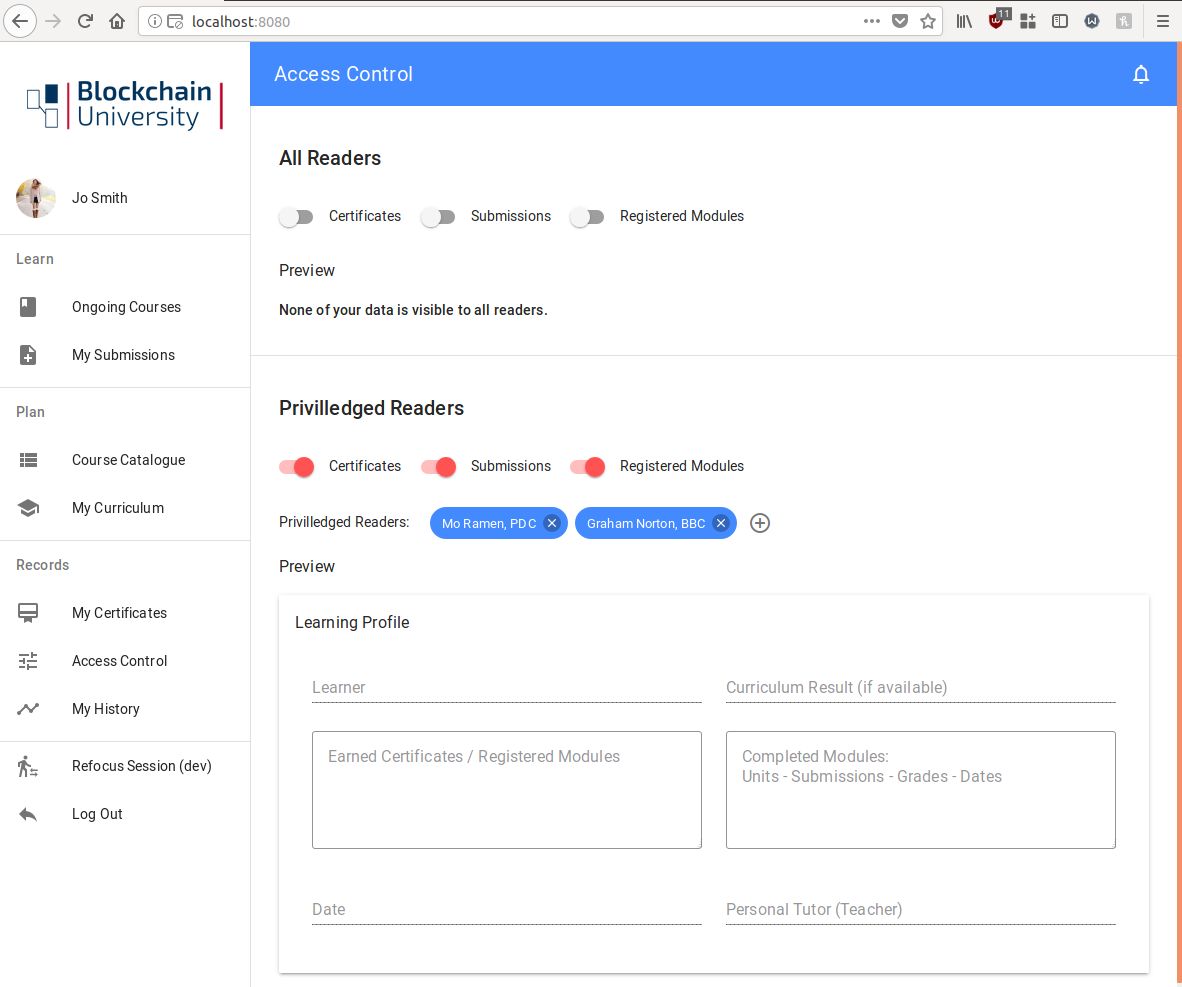
\includegraphics[width=1.0\textwidth]{Learner_AC}
	\caption[Learner Application Access Control Page]
	{Learner Application Access Control Page}
	\label{fig:Learner_AC}
\end{figure}

\clearpage
\subsection{Teacher Application}

The Teacher application was created as a fork of the Learner application. 
The source code of this application is tracked and hosted at 
\href{https://github.com/dtylam/moocon-teacher-client}{\underline{github.com/dtylam/moocon-teacher-client}}.
Only one iteration was completed by the end of the project, as this application was built after requirements gathering interviews.

Below are some annotated screenshots of this application (Figures \ref{fig:Teacher_createcourse} to 
\ref{fig:Teacher_marking}). [annotations TODO]

\begin{figure}[!ht]
	\centering
	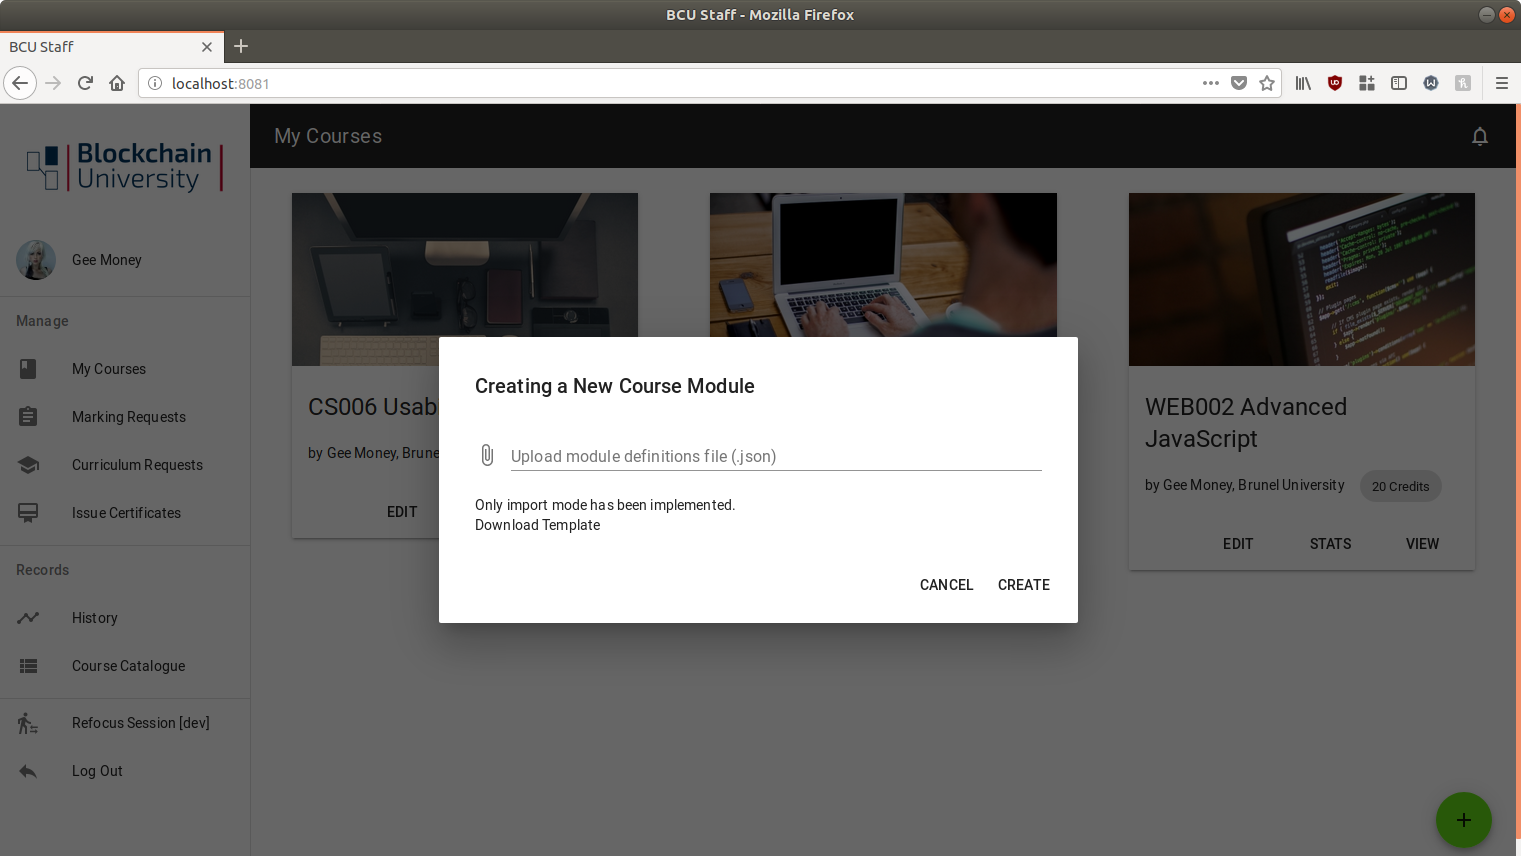
\includegraphics[width=1.0\textwidth]{Teacher_createcourse}
	\caption[Teacher Application My Courses Page]
	{Teacher Application My Courses Page}
	\label{fig:Teacher_createcourse}
\end{figure}

\begin{figure}[!ht]
	\centering
	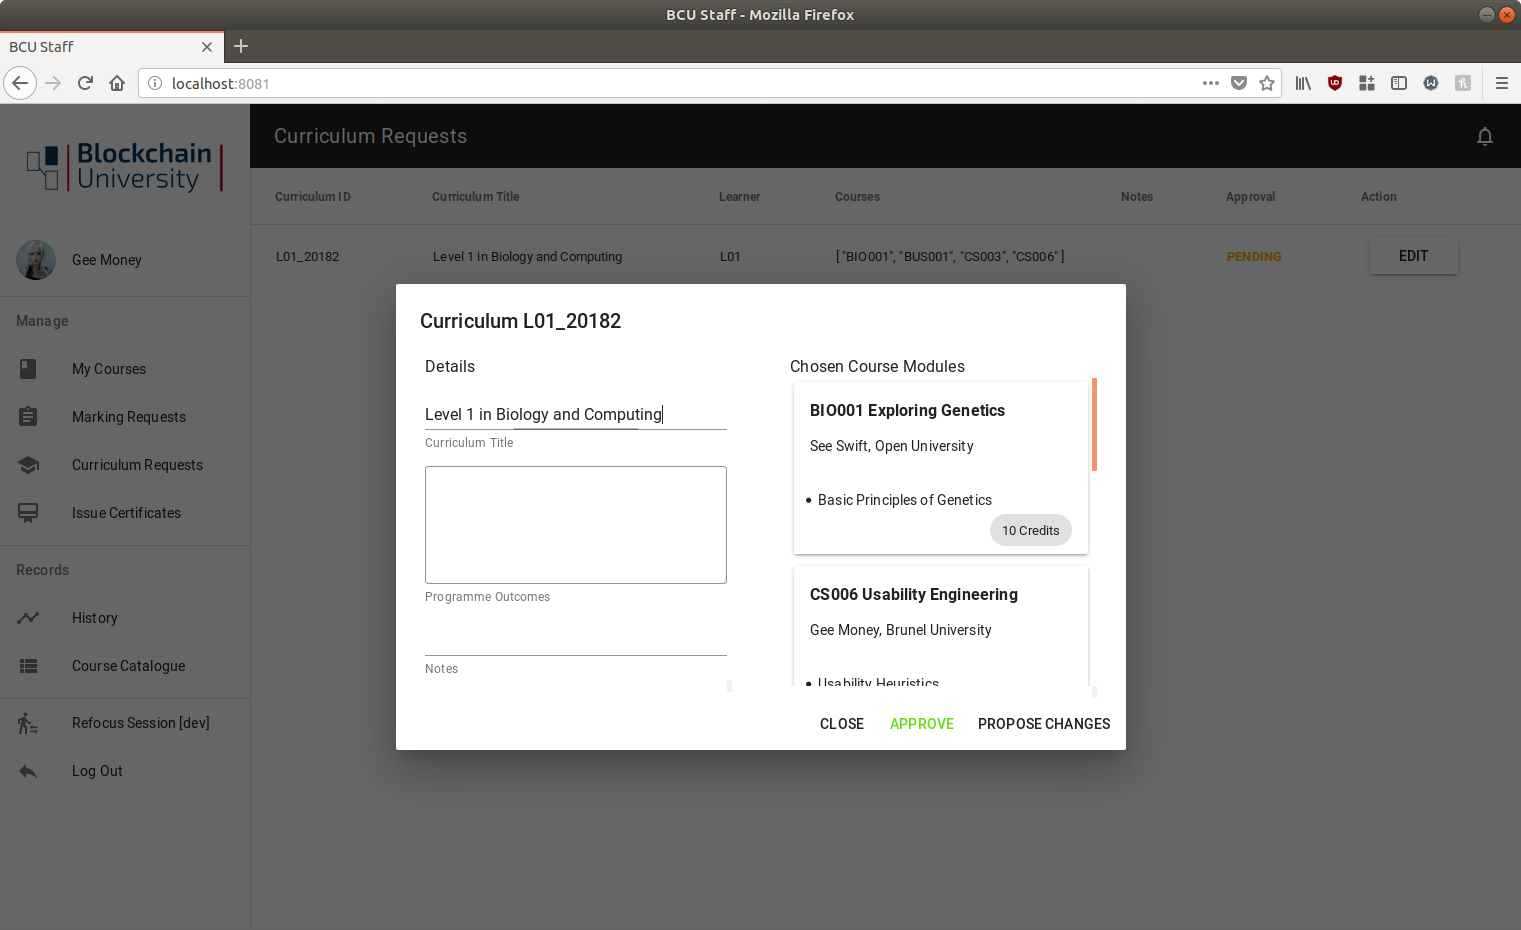
\includegraphics[width=1.0\textwidth]{Teacher_approvecurr}
	\caption[Teacher Application Curriculum Requests Page]
	{Teacher Application Curriculum Requests Page}
	\label{fig:Teacher_approvecurr}
\end{figure}

\begin{figure}[!ht]
	\centering
	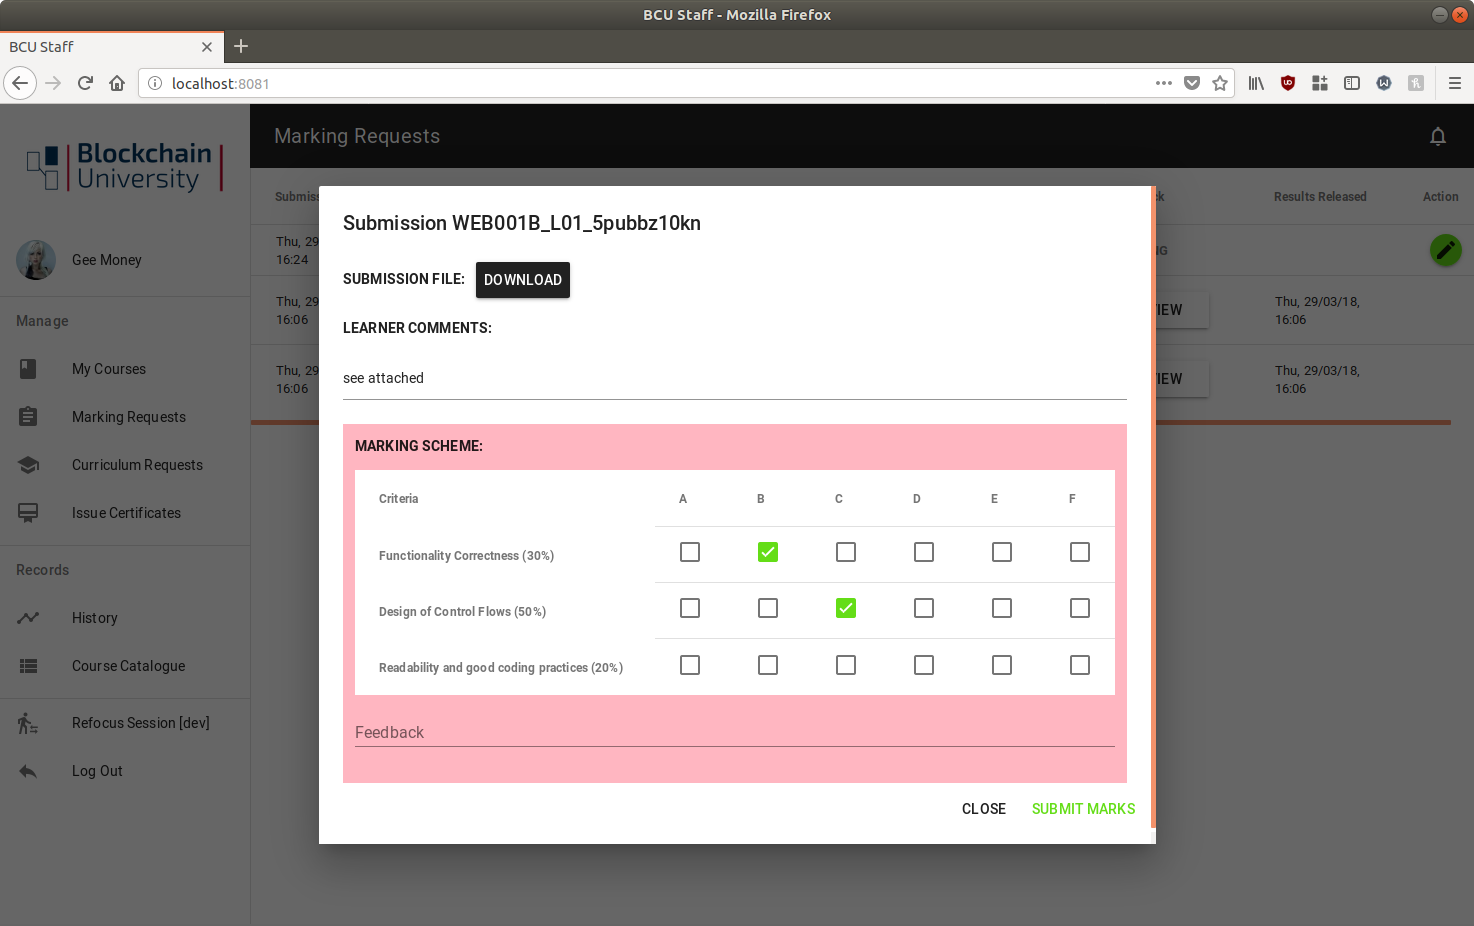
\includegraphics[width=1.0\textwidth]{Teacher_marking}
	\caption[Teacher Application Marking Requests Page]
	{Teacher Application Marking Requests Page}
	\label{fig:Teacher_marking}
\end{figure}

\clearpage
\section{Test-Driven Development}

At the early stages of this project, an attempt at test-driven development was made. 
Support for unit testing is built-in for Hyperledger Composer with popular JavaScript testing frameworks Mocha and Chai.
Unit tests were written before writing the code for transactions.

With the Hyperledger Composer 0.16 upgrade, the test scripts stopped working as 
the method for connecting to the blockchain network has changed. This complication 
rendered the tests written useless, and attempts were made to port the tests over 
to work in the updated framework but were not immediately successful. In the interest of 
time, test-driven development was abandoned.

At the time of abandoning these efforts, three unit tests were written targeting transactions, 
and two were passing. One asserts that a learner can subscribe to a course, 
and the other asserts that a learner can add a new submission. 
These tests can be found at: \href{https://github.com/dtylam/moocon-alpha/blob/master/test/test_end2end.js}
{\underline{github.com/dtylam/moocon-alpha/.../test\_end2end.js}}.

\section{Limitations, Outstanding Issues and Features}

\subsection{Limitations}

The frameworks used have some notable limitations:
\vspace{0.25cm}\\
\textbf{Limitation 1: Blockchain Events were broadcasted network-wide without access control filters.}

Some Events are only targeted at a particular individual but all of the peers will receive it.
For example, only the proposing \textit{Learner} and their personal tutor \textit{Teacher} should 
be receiving the notification that a curriculum has been proposed. Currently, all peers across the 
blockchain receive these notifications, they are only hidden at the client application level.

This is a limitation of Hyperledger Composer, which does not provide ways to limit the scope of an \textit{Event}.
It would cause privacy issues for a real-world system, as any actor on the blockchain could potentially 
listen to these \textit{Events} and attempt to create a partial view of user histories.
\vspace{0.25cm}\\
\textbf{Limitation 2: Client applications login sessions do not persist.}

Built with the simple Vue.js framework which does not have built-in caching capabilities 
(that is included in a separate VueX framework), when the page is reloaded the login session 
is automatically ended. This could frustrate real-world users but is accepted as a limitation 
for this demonstrator.

\subsection{Outstanding Issues}

With a finite amount of time dedicated to development, a number of issues remain:
\vspace{0.25cm}\\
\textbf{Issue 1: Notification icon in client applications are not changing when new notifications arrive.}

The JavaScript function that receives Websocket messages (the web standard channel where new 
blockchain Events are broadcasted) was written in vanilla JavaScript outside of the Vue.js 
framework. The Vue.js conditional block that controls the notification icon is not responsive.
\vspace{0.25cm}\\
\textbf{Issue 2: Main menu in learner application freezes after adding a new Viva booking submission.}

This is a Heisenbug which appears only sometimes when a full live demo flow is performed. 
For a proof-of-concept demonstrator, the stability of the application is not the most important factor 
and priority was not given to solving this issue.

\subsection{Outstanding Features}

Several features were not built in time for the demonstrator system evaluation.
Most of these features were not prioritised as "Must Have" previously in Chapter 4.2:

\begin{itemize}
	\setlength\itemsep{0em}	
	\item GenCertificate transaction (chaincode)
	\item My Certificate page for Learner application (UI)
	\item Certificate Requests page for Teacher application (UI)	
	\item Feedback viewing dialogue for client applications (UI)
\end{itemize}

\section*{Summary}

A working blockchain network, a client application for learners, and another for teachers 
were successfully built. 

A demonstration workflow was created as the implementation phase came to an end to allow 
time for user evaluation. The previously mentioned video at 
\href{https://youtu.be/FUMBn6wPG5M}{\underline{youtube.com/FUMBn6wPG5M}} 
was recorded following the same steps as the user evaluation demonstration.

The following chapter will discuss evaluation further.
%!TEX root = ../thesis.tex
%*******************************************************************************
%****************************** Seventh Chapter **********************************
%*******************************************************************************
\chapter{Conclusion}

\section{Future Work}
and here I write more \dots


%!TEX root = ../thesis.tex
%*******************************************************************************
%****************************** Seventh Chapter **********************************
%*******************************************************************************
\chapter{Conclusion}

\section{Work Completed}

Deliverables:

Aims and Objectives:

- proved that Smart Contracts can bring value to assessment and personalisation

\section{Limitations}

- limitations of development frameworks

- human limitations: the system has the potential to improve interactions but depends on quality of human inputs 

- explicit description of learning outcomes, programme specifications, grade descriptors is not enough, teachers should
engaging students in activities pre-assessment intervention \citep{bryan2006innovative}

- public awareness

\section{Future Work}

% - tests embedded in smart contracts instead of rest calls, which may not always be available

- consensus model for double marking, etc

-- reputation model and community policing build trust

-- who issues the award? different modes and uses. 

-- arbitration, appeals and extenuating circumstances



and here I write more \dots

https://www.timeshighereducation.com/news/oxford-academics-launch-worlds-first-blockchain-university
\end{spacing}
% ********************************** Back Matter *******************************
% Backmatter should be commented out, if you are using appendices after References
%\backmatter

% ********************************** Bibliography ******************************
\begin{spacing}{0.9}

% To use the conventional natbib style referencing
% Bibliography style previews: http://nodonn.tipido.net/bibstyle.php
% Reference styles: http://sites.stat.psu.edu/~surajit/present/bib.htm

\bibliographystyle{apalike}
%\bibliographystyle{unsrt} % Use for unsorted references  
%\bibliographystyle{plainnat} % use this to have URLs listed in References
\cleardoublepage
\bibliography{References/references} % Path to your References.bib file


% If you would like to use BibLaTeX for your references, pass `custombib' as
% an option in the document class. The location of 'reference.bib' should be
% specified in the preamble.tex file in the custombib section.
% Comment out the lines related to natbib above and uncomment the following line.

%\printbibliography[heading=bibintoc, title={References}]

\end{spacing}

% ********************************** Appendices ********************************

\begin{appendices} % Using appendices environment for more functunality

%!TEX root = ../thesis.tex
% ******************************* Thesis Appendix A ****************************
\chapter{Reflection} 

This project has driven me to grow in three main areas: research, project management, 
and technical skills.

\section{Research Skills}

\section{Project Management Skills}

\section{Technical Skills}

%!TEX root = ../thesis.tex
% ******************************* Thesis Appendix B ********************************

\chapter{Installing the CUED class file}

\LaTeX.cls files can be accessed system-wide when they are placed in the
<texmf>/tex/latex directory, where <texmf> is the root directory of the user’s \TeX installation. On systems that have a local texmf tree (<texmflocal>), which
may be named ``texmf-local'' or ``localtexmf'', it may be advisable to install packages in <texmflocal>, rather than <texmf> as the contents of the former, unlike that of the latter, are preserved after the \LaTeX system is reinstalled and/or upgraded.

It is recommended that the user create a subdirectory <texmf>/tex/latex/CUED for all CUED related \LaTeX class and package files. On some \LaTeX systems, the directory look-up tables will need to be refreshed after making additions or deletions to the system files. For \TeX Live systems this is accomplished via executing ``texhash'' as root. MIK\TeX users can run ``initexmf -u'' to accomplish the same thing.

Users not willing or able to install the files system-wide can install them in their personal directories, but will then have to provide the path (full or relative) in addition to the filename when referring to them in \LaTeX.



\end{appendices}

% *************************************** Index ********************************
\printthesisindex % If index is present

\end{document}
